\documentclass{beamer}
\usetheme{Frankfurt}

\usepackage{listings}
\usepackage{fancyvrb}

\newcommand{\todo}[1]{\alert{TODO #1}}

\setbeamertemplate{footline}[frame number]

\title{Operating Systems}
\subtitle{Lecture 2 \\ Computer Security DD2395}
\author[R. Guanciale]{
  Roberto Guanciale\\
  robertog@kth.se
}
\date{2016-11-04}
\begin{document}

\maketitle

\begin{frame}{Roberto Guanciale}
  \begin{itemize}
    \item Assistant professor \alert{Computer Security}
    \item Research interest in \alert{Formal Verification}
      \begin{itemize}
        \item Hack-proof Operating Systems
      \end{itemize}
    \item Enthusiast software developer
    \item robertog@kth.se
    \item Office: level 5, room 4525
    \item You are welcomed (no booking required, no fee)
    \begin{itemize}
      \item Wednesday 14:00-15:00
    \end{itemize}
  \end{itemize}
\end{frame}

\begin{frame}{About you}
  \begin{itemize}
    \item University:
    \item Program:
    \item Computer architecture:
    \item Programming language:
    \item Operating Systems:
  \end{itemize}
\end{frame}

\begin{frame}{Interactive lecture}
  \center{
    www.guancio.com\\
    
\includegraphics[width=0.5\linewidth]{qrcode}
  }
\end{frame}

\begin{frame}{Main questions}
  \begin{itemize}
    \item How can we run Chrome on a modern architecture?
    \item How can we isolate Chrome from LibreOffice?
    \item How can we run multiple instances of Chrome?
    \item How can we run Chrome on two phones with
      two different network controllers?
  \end{itemize}
\end{frame}

\begin{frame}{Operating Systems}
  \begin{itemize}
  \item An OS is a program that acts an intermediary
    between applications and computer hardware
\alert{Image of app, OS, Devices}
  \item Simplify the execution of applications.
  \item Allow sharing of hardware and software resources.
  \item Make application software portable and versatile.
  \item Provide isolation, security and protection among
    applications.
  \end{itemize}
\end{frame}

\begin{frame}{Example of OSes}
  \begin{itemize}
  \item Windows/Linux/OS X ($\sim$ 50 milions LOC)
  \item<2-> Android/iOS ($\sim$ 50 milions LOC)
  \item<3-> S40 ($\sim$ 1 milions LOC)
  \item<4-> Free RTOS ($\sim$ 10 000 LOC)
  \item<5-> L4 microkernel ($\sim$ 10 000 LOC)
  \item<6-> Automotive
  \item<7-> Nuclear power plants/Airplanes/Drones
  \end{itemize}
\end{frame}

\begin{frame}{OS by example}
  How can we run Chrome on a modern CPU?
\end{frame}

\begin{frame}[t]{HW architecture}
  \begin{itemize}
  \item Common architectures x86, x64, ARM, MIPS, PowerPC
  \item<3-> Program stored in memory
  \item<4-> Program Counter (PC): address of the current instruction
  \end{itemize}
\center{
\only<1> {
  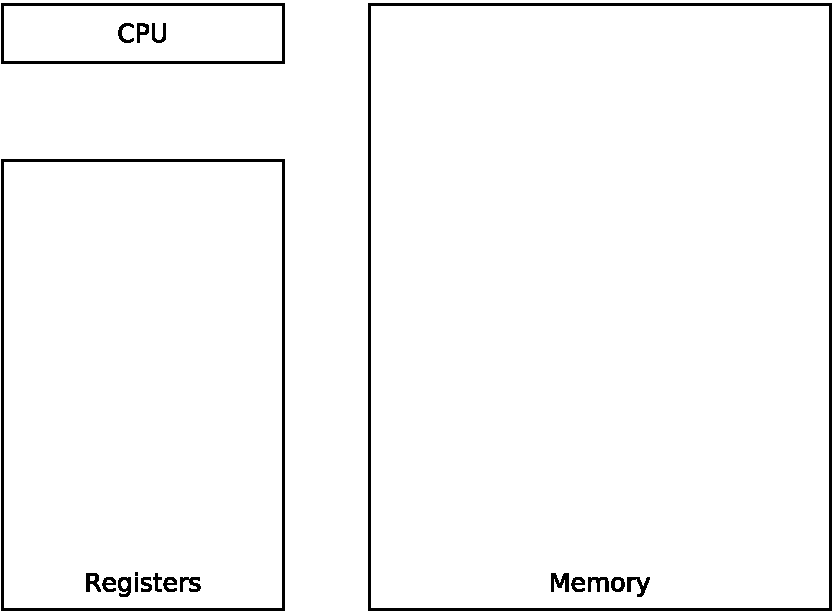
\includegraphics[width=0.5\linewidth]{hw-0}
}
\only<2> {
  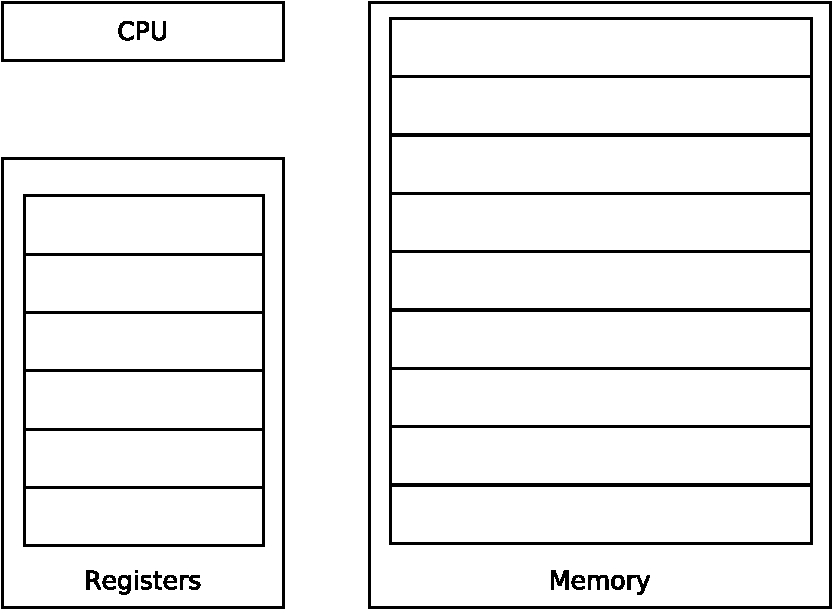
\includegraphics[width=0.5\linewidth]{hw-1}
}
\only<3> {
  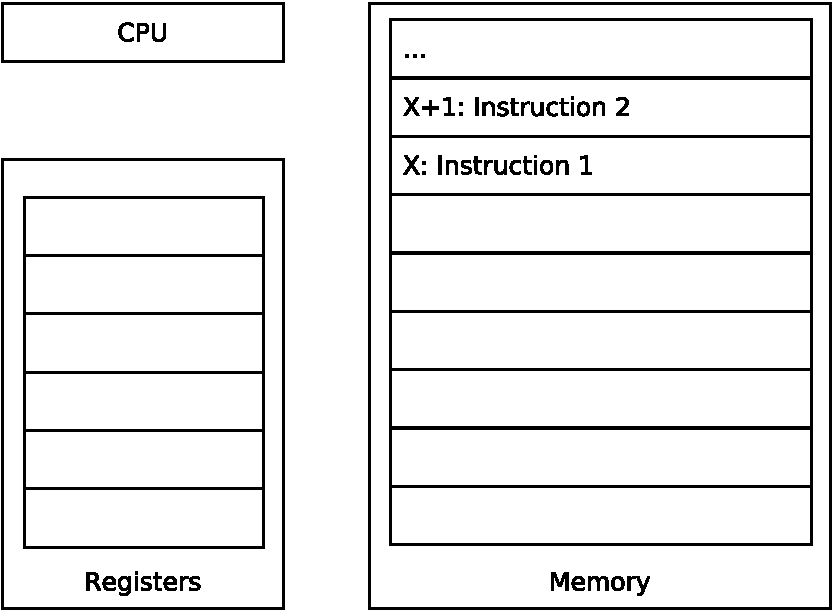
\includegraphics[width=0.5\linewidth]{hw-2}
}
\only<4> {
  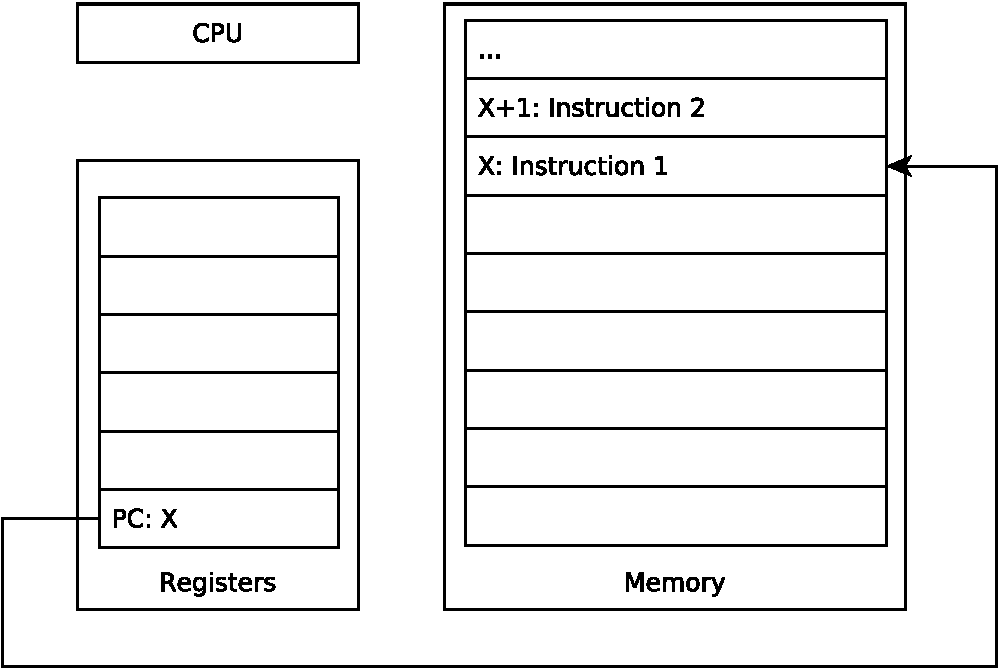
\includegraphics[width=0.6\linewidth]{hw-3}
}
    \only<5> {
  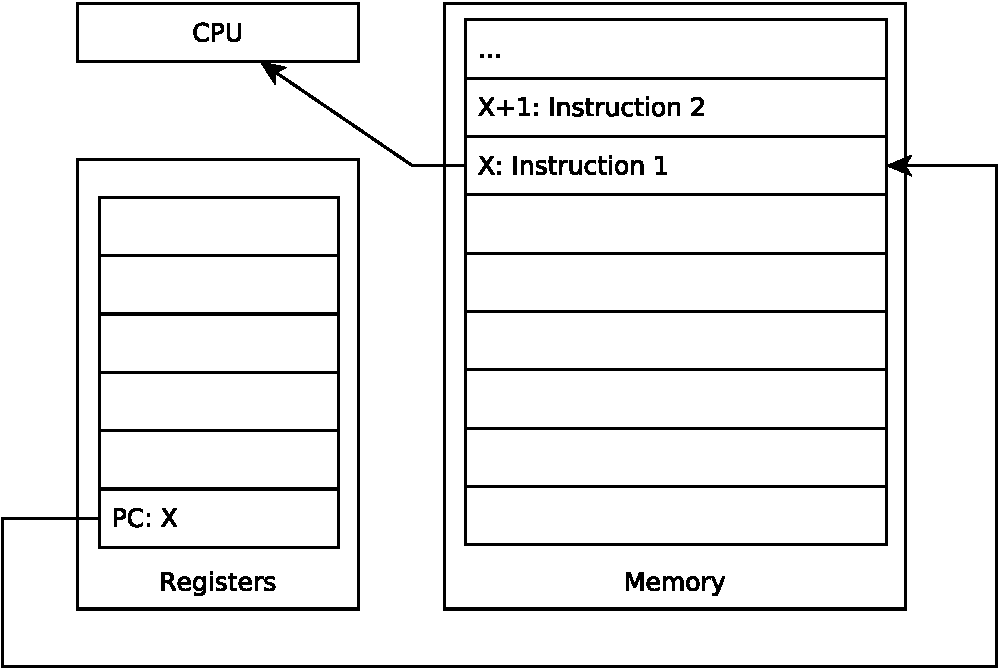
\includegraphics[width=0.6\linewidth]{hw-4}
}
    \only<6> {
  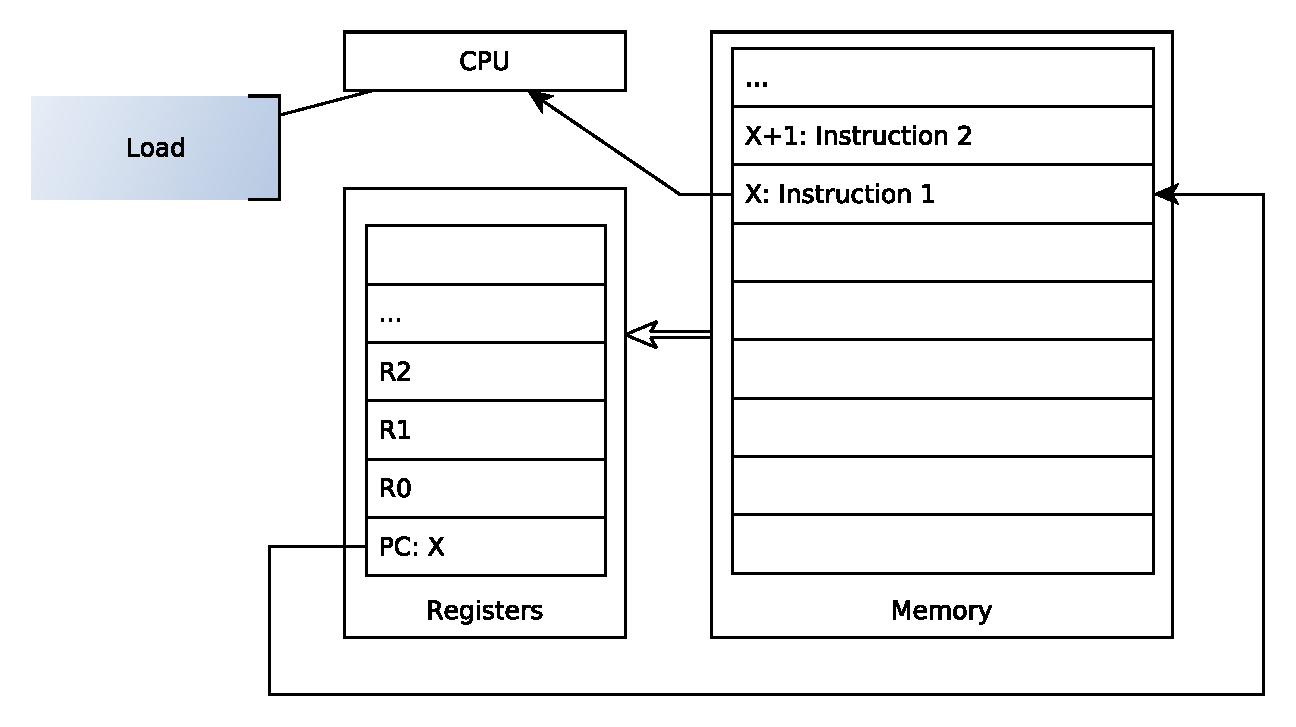
\includegraphics[width=0.8\linewidth]{hw-5}
}
    \only<7> {
  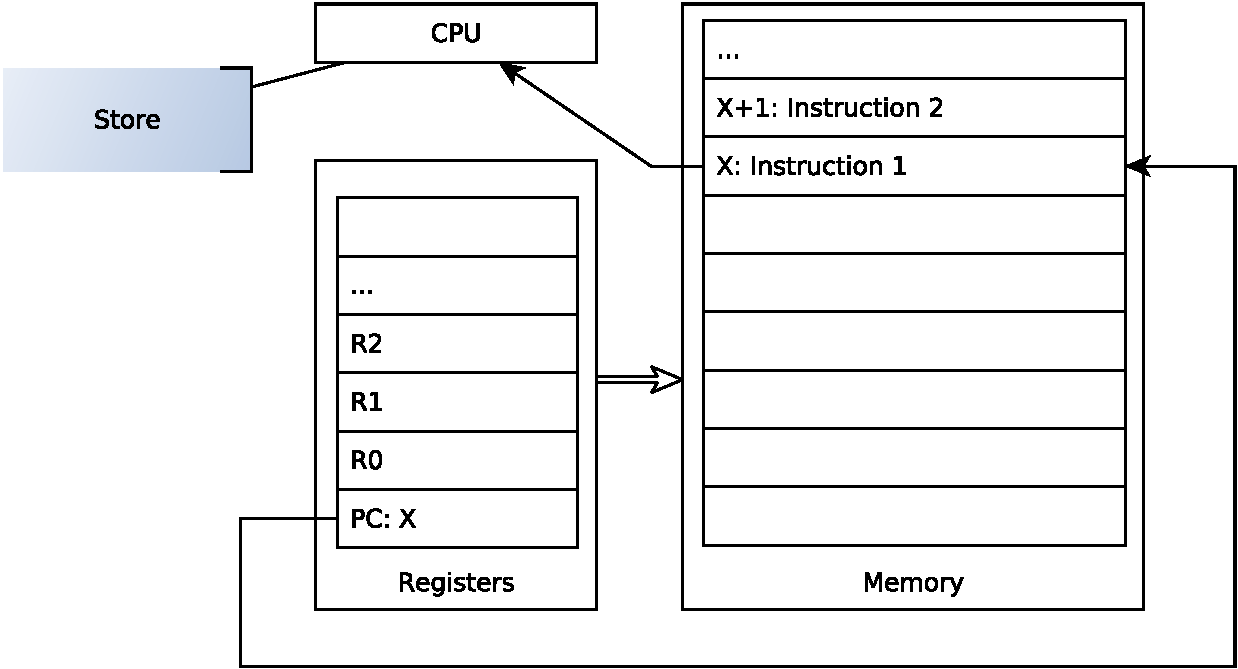
\includegraphics[width=0.8\linewidth]{hw-6}
}
    \only<8> {
  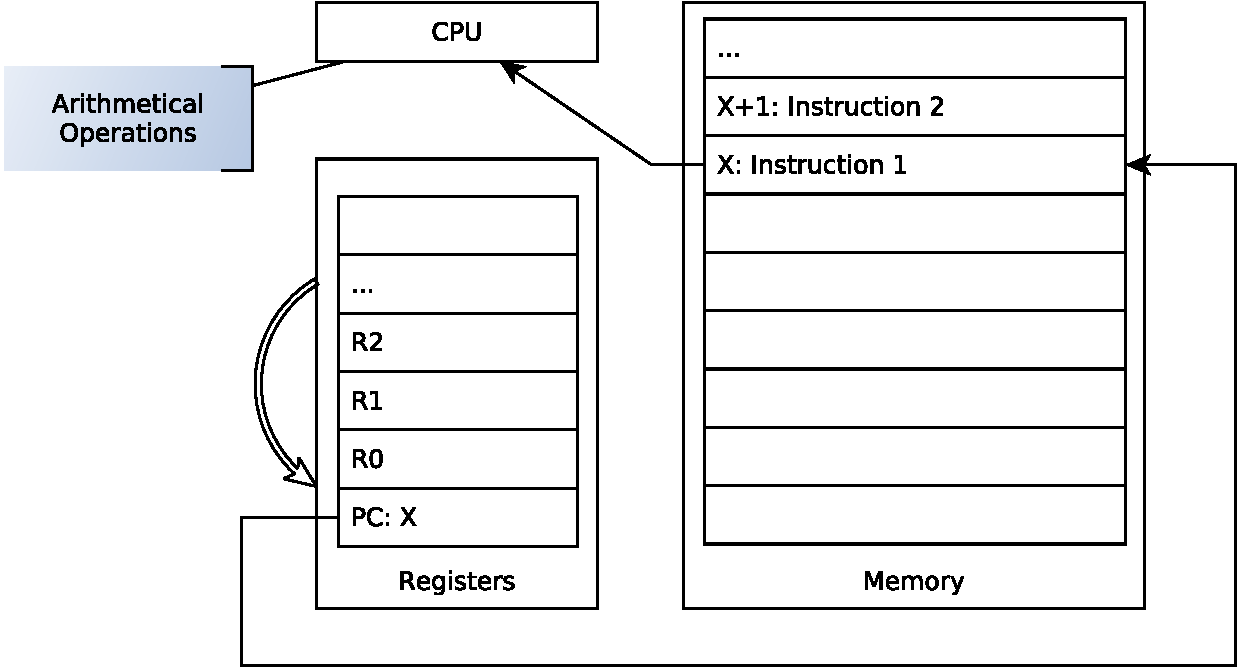
\includegraphics[width=0.8\linewidth]{hw-7}
}
    \only<9> {
  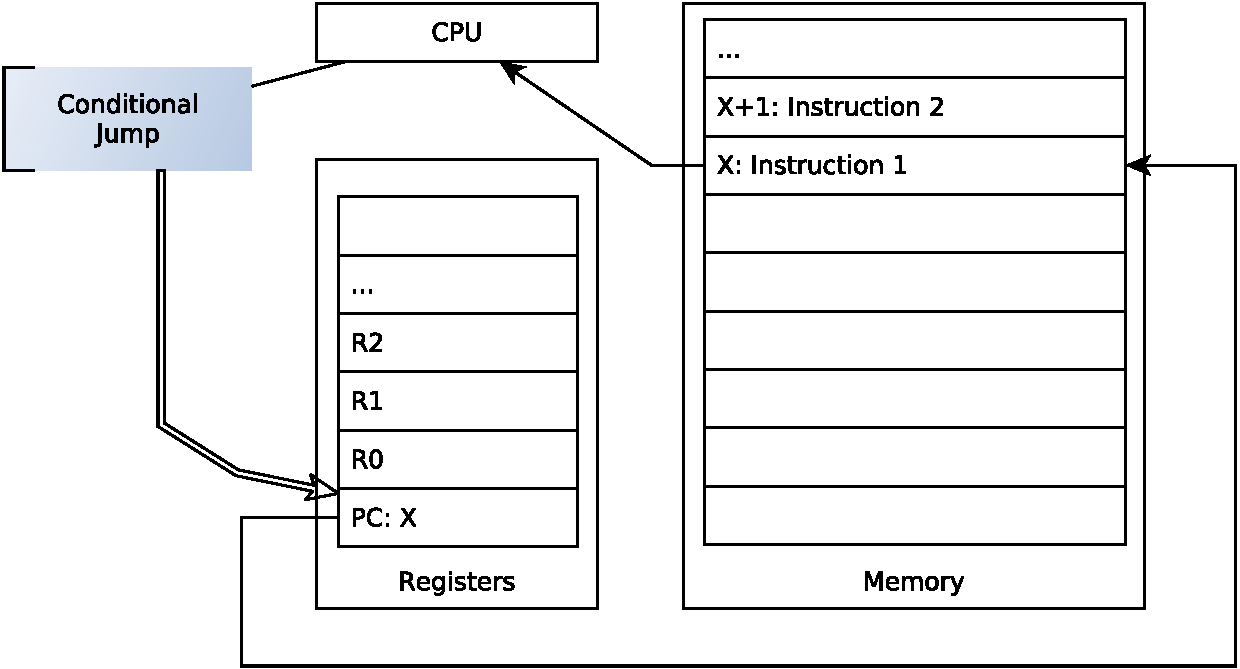
\includegraphics[width=0.8\linewidth]{hw-8}
}}
\end{frame}

\begin{frame}[fragile]{Application memory}
\begin{Verbatim}[fontsize=\small]

int x;
int * hello(int y) {
  int * res = malloc(8);
  res[0] = x + 10;
  res[1] = y + x;
  return res;
}
\end{Verbatim}
\end{frame}

\begin{frame}[fragile]{Application memory}
\begin{Verbatim}[fontsize=\small]
                        class Example {
int x;                     static int x;
int * hello(int y) {       int[] hello(int y) {
  int * res = malloc(8);      int[] res = new int[2];
  res[0] = x + 10;            res[0] = x + 10;
  res[1] = y + x;             res[1] = y + x;
  return res;                 return res;
}                          }
\end{Verbatim}
\end{frame}

\begin{frame}[t]{Application Memory}
\center
{    \only<1-2> {
  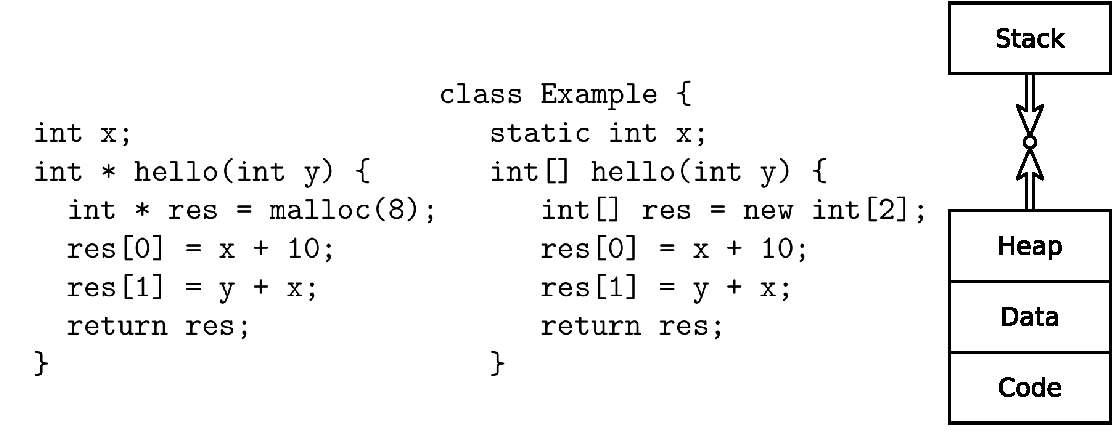
\includegraphics[width=0.9\linewidth]{code1}
}
  \only<2> {
    Discuss five minutes with your colleagues\\
  }
  \only<2> {
    Where each element is allocated?
  }
    \only<3> {
  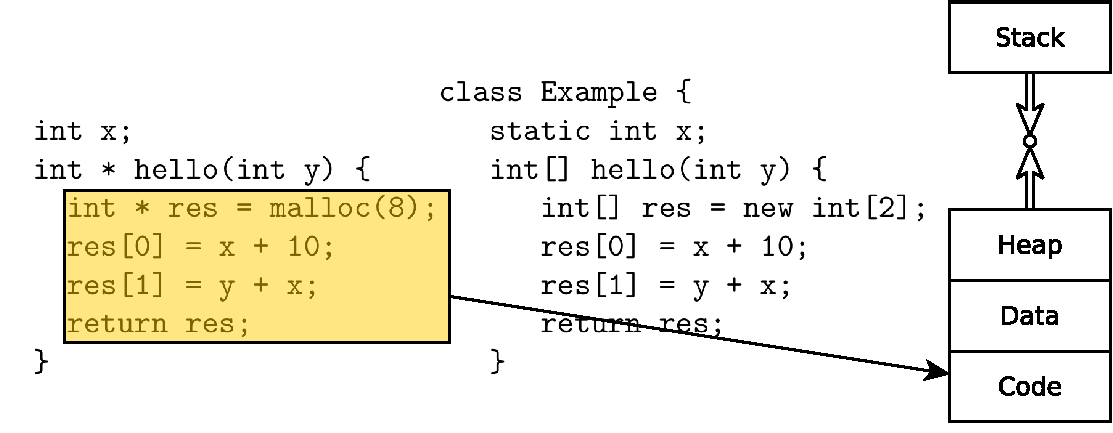
\includegraphics[width=0.9\linewidth]{code2}
}
    \only<4> {
  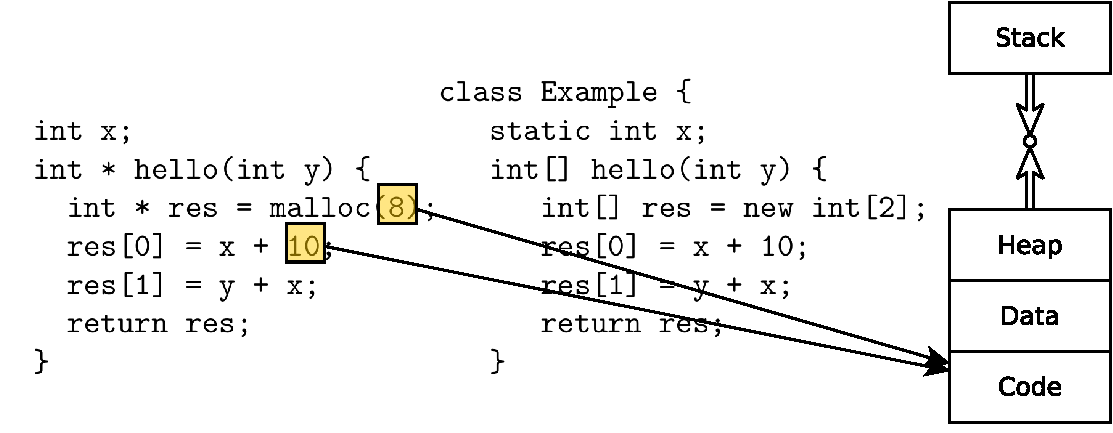
\includegraphics[width=0.9\linewidth]{code3}
}
    \only<5> {
  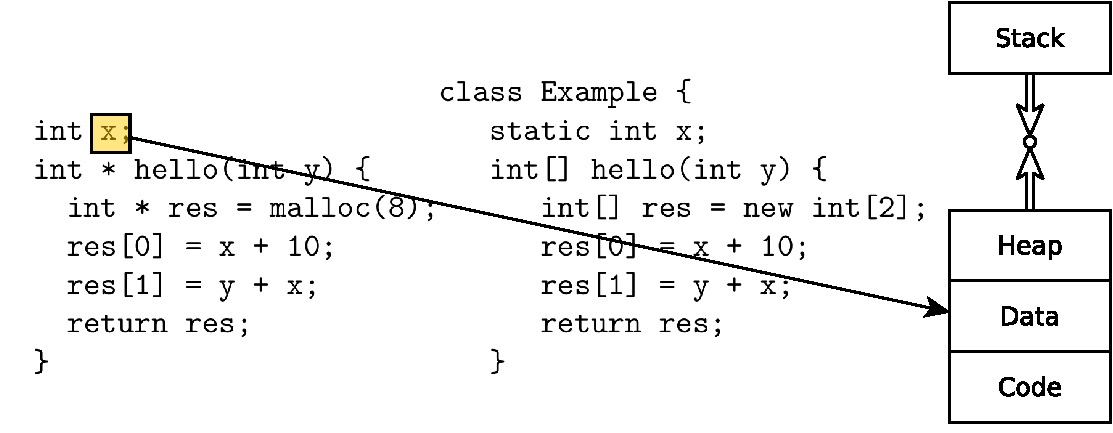
\includegraphics[width=0.9\linewidth]{code4}
}
    \only<6> {
  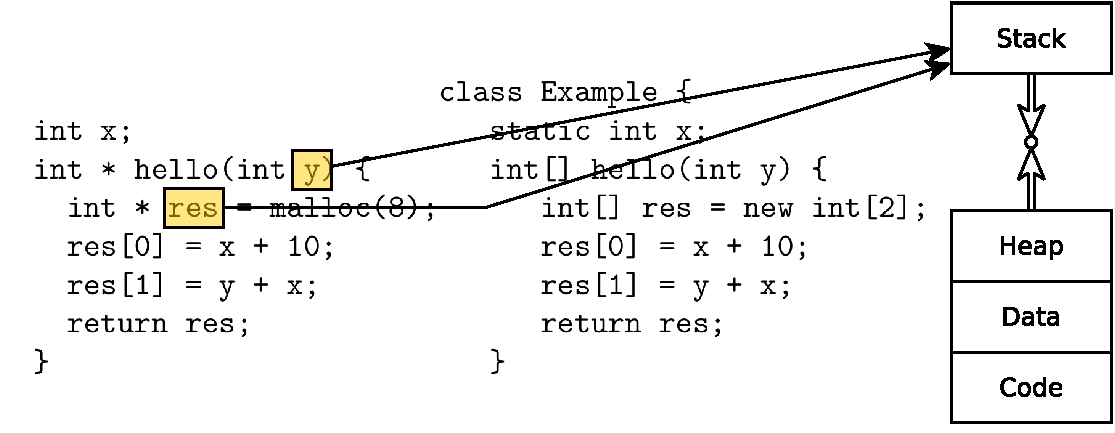
\includegraphics[width=0.9\linewidth]{code5}
}
    \only<7> {
  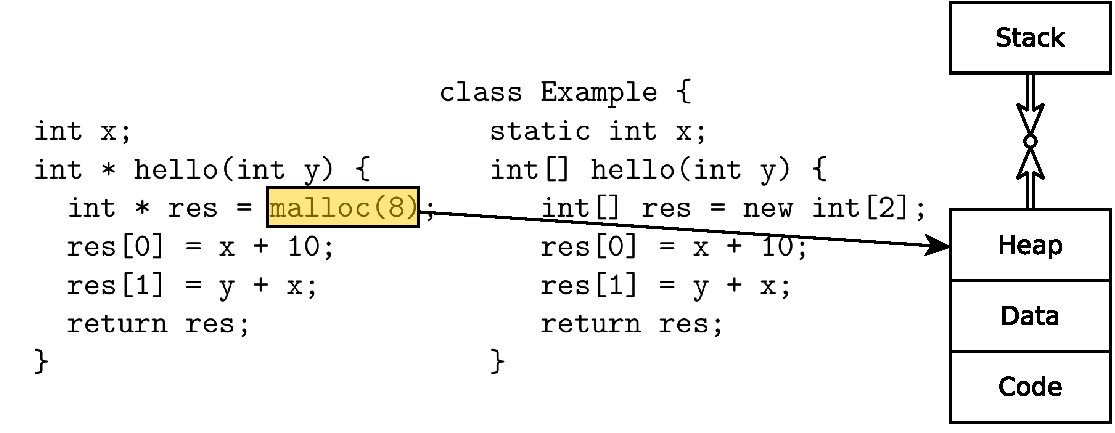
\includegraphics[width=0.9\linewidth]{code6}
}
    \only<8> {
  \begin{itemize}
    \item Stack Pointer points to the bottom of the stack
      \\[20pt]
  \end{itemize}
  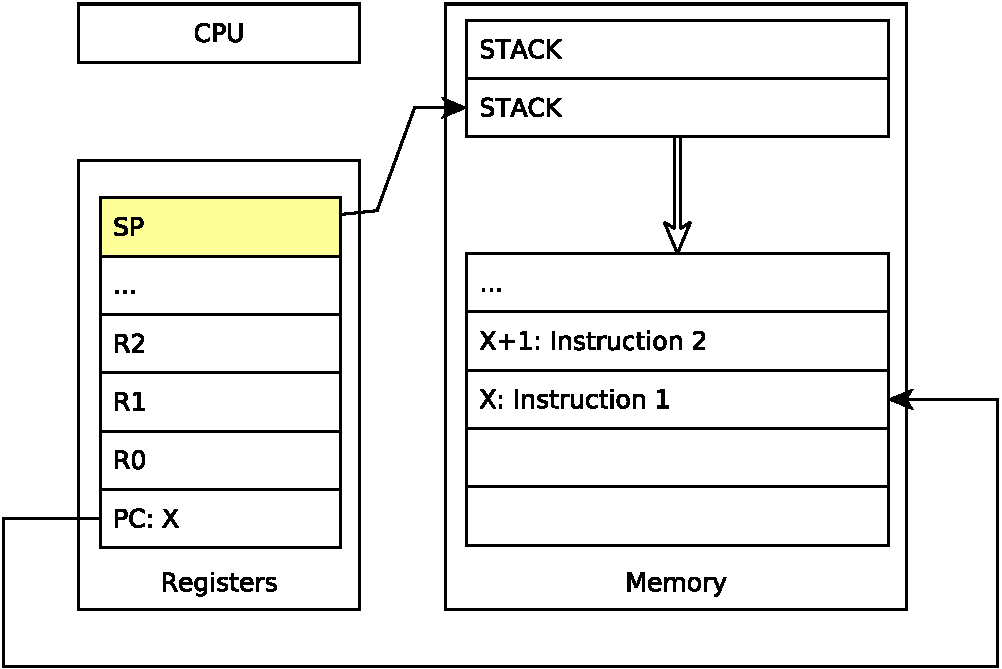
\includegraphics[width=0.6\linewidth]{stack}
}}
\end{frame}



\begin{frame}{Virtual Memory}
  \begin{itemize}
  \item Modern systems do not use directly physical addresses
    \begin{itemize}
    \item Free to allocate applications in different memory area
    \item Free to dynamically allocate memory for processes
    \item Run the same software in systems with 1GB or 2 GB of memory
    \item Run the same binary as two distinct processes
    \end{itemize}
  \item<2-> Virtual memory
    \begin{itemize}
    \item SW uses virtual addresses
    \item HW configuration maps virtual addresses to physical addresses
    \item HW configuration updatable
    \item HW mechanism is called Memory Management Unit
    \end{itemize}
  \end{itemize}
\end{frame}

\begin{frame}{Virtual Memory}
  \begin{center}
  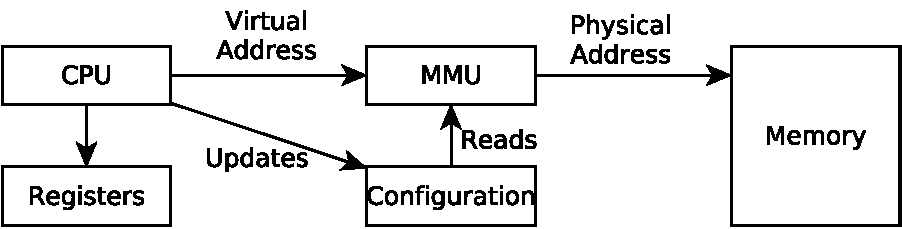
\includegraphics[width=0.5\linewidth]{mmu1}\\[30pt]
    \only<1> {
  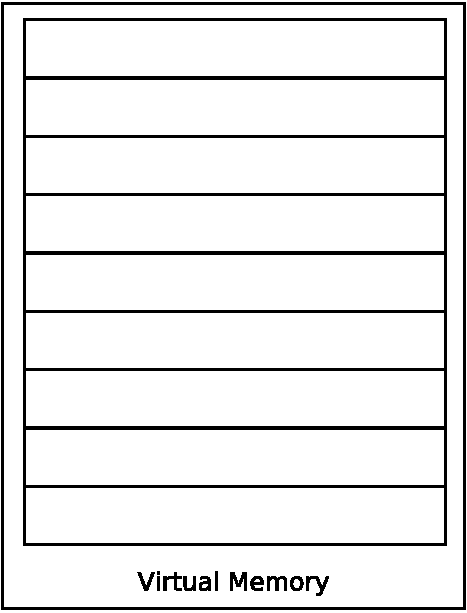
\includegraphics[width=0.2\linewidth]{mmu2}
}
    \only<2> {
  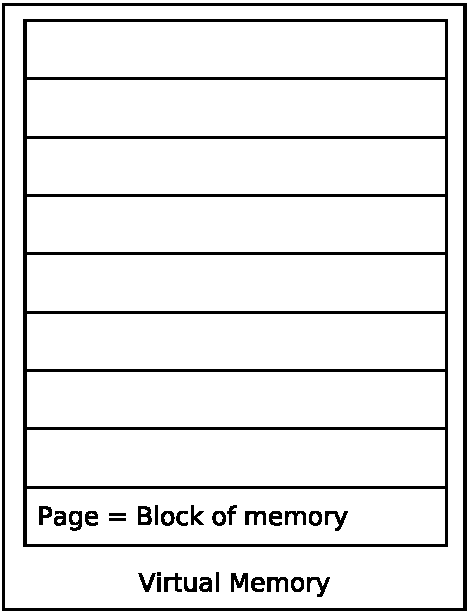
\includegraphics[width=0.2\linewidth]{mmu3}
}
    \only<3> {
  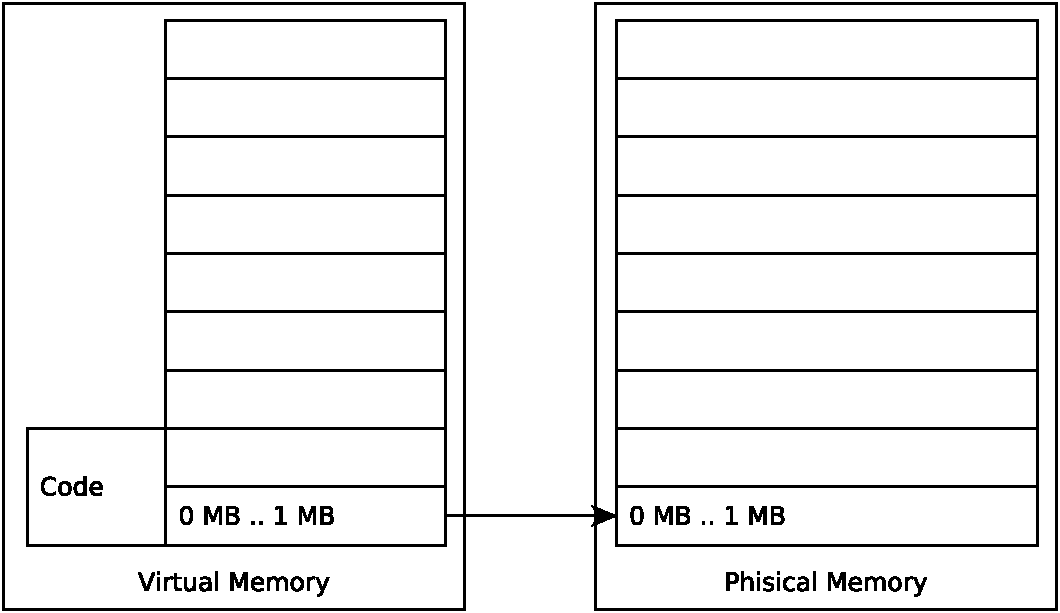
\includegraphics[width=0.5\linewidth]{mmu4}
}
    \only<4> {
  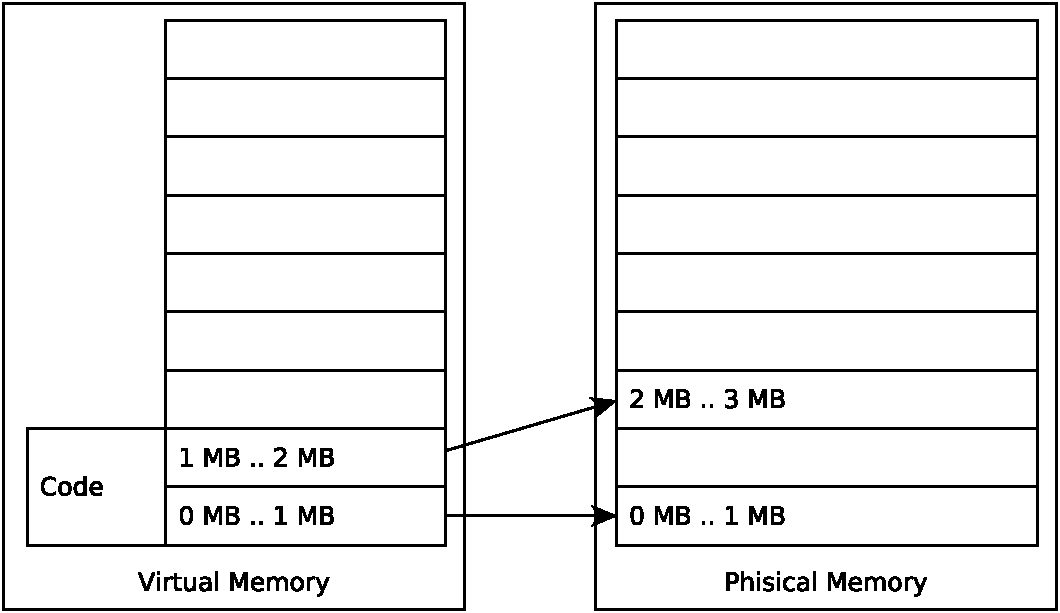
\includegraphics[width=0.5\linewidth]{mmu5}
}
    \only<5> {
  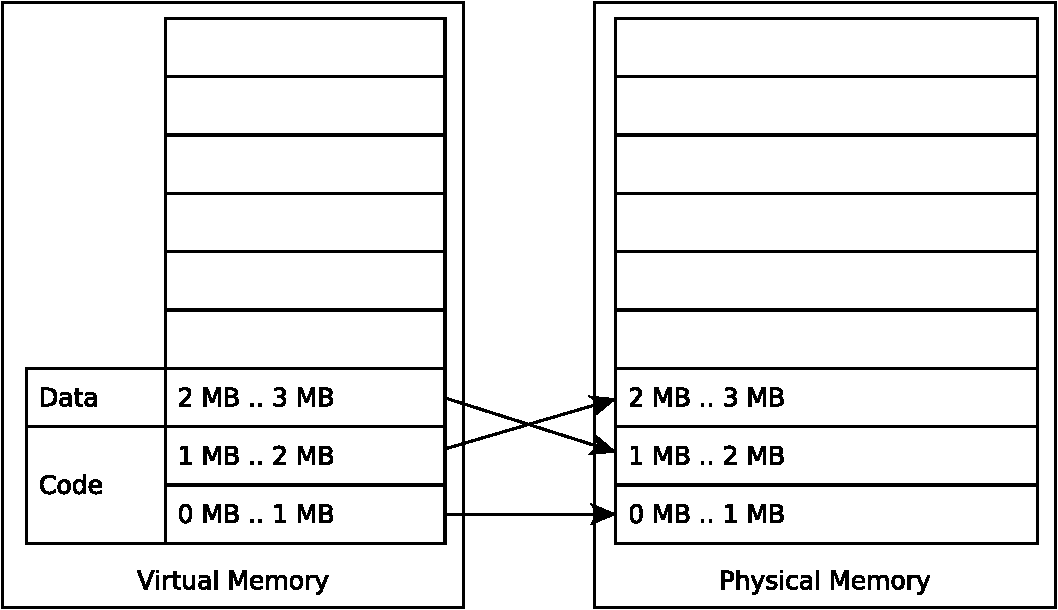
\includegraphics[width=0.5\linewidth]{mmu6}
}
    \only<6> {
  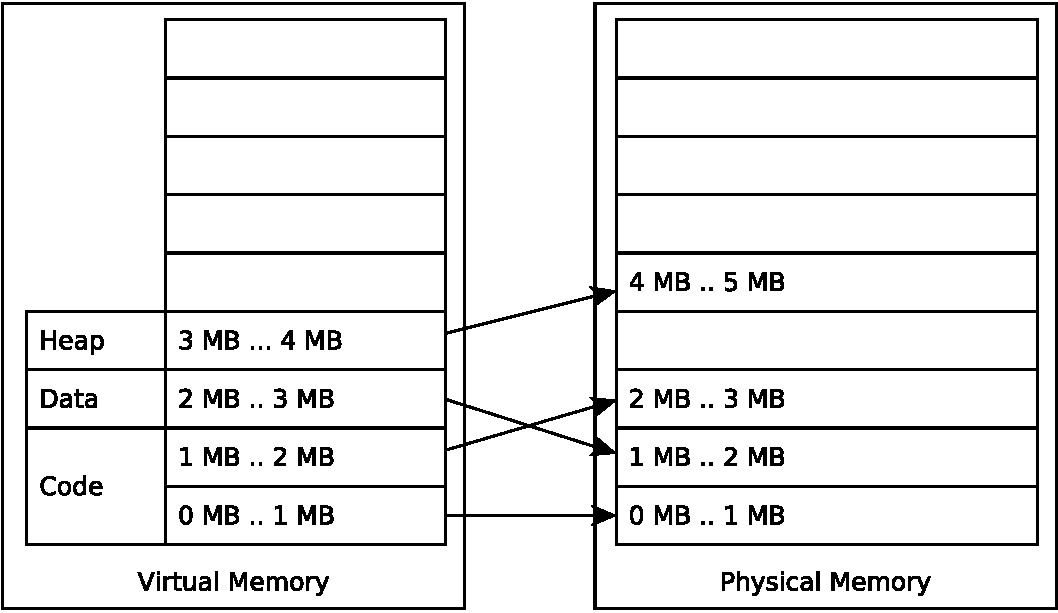
\includegraphics[width=0.5\linewidth]{mmu7}
}
    \only<7> {
  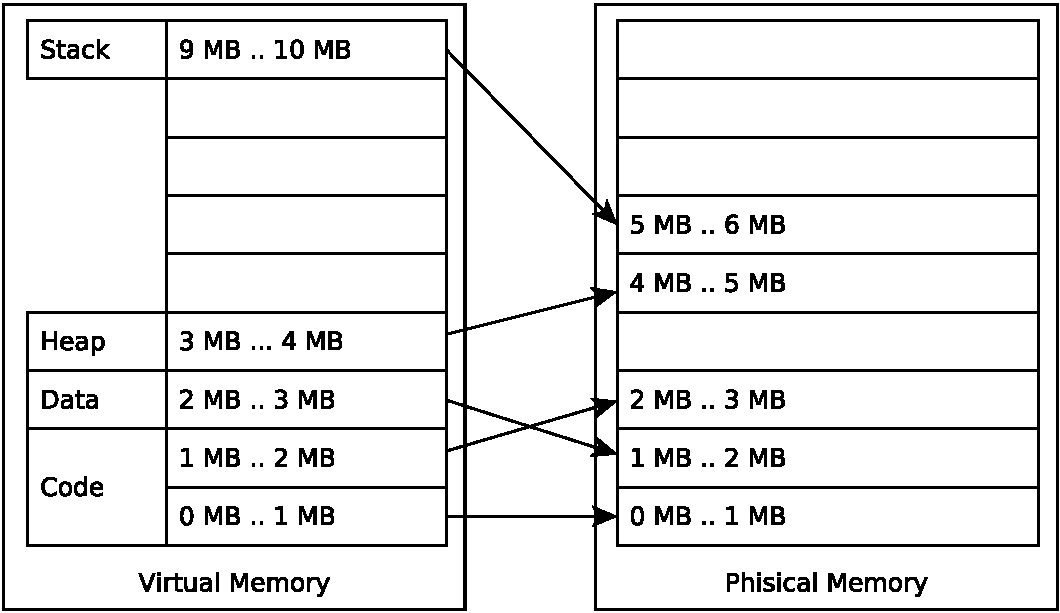
\includegraphics[width=0.5\linewidth]{mmu8}
}
    \only<8> {
  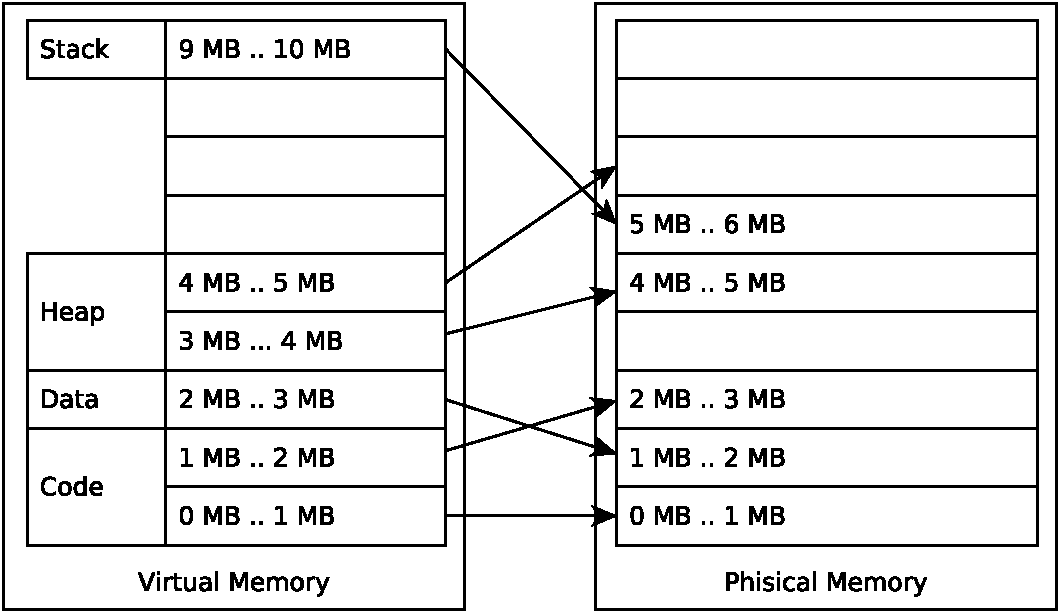
\includegraphics[width=0.5\linewidth]{mmu9}
}
    \only<9> {
  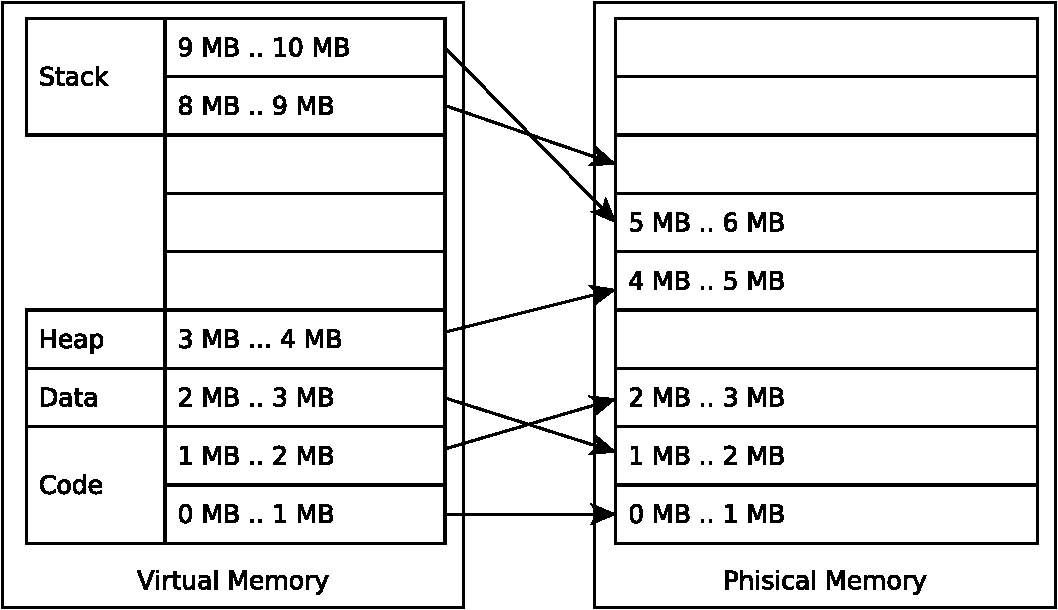
\includegraphics[width=0.5\linewidth]{mmu10}
}
  \end{center}
\end{frame}





\begin{frame}{OS by example: 2}
  \begin{itemize}
    \item How can we isolate Chrome from LibreOffice?
    \item<2-> Two types of resources:
      \begin{itemize}
        \item registers \only<3>{$\Rightarrow$ multiplex}
        \item memory \only<3>{$\Rightarrow$ isolation}
      \end{itemize}
    \item <3-> One of the main tasks of an OS
  \end{itemize}
\end{frame}


\begin{frame}{Context switch}
  \begin{center}
    \only<1> {
  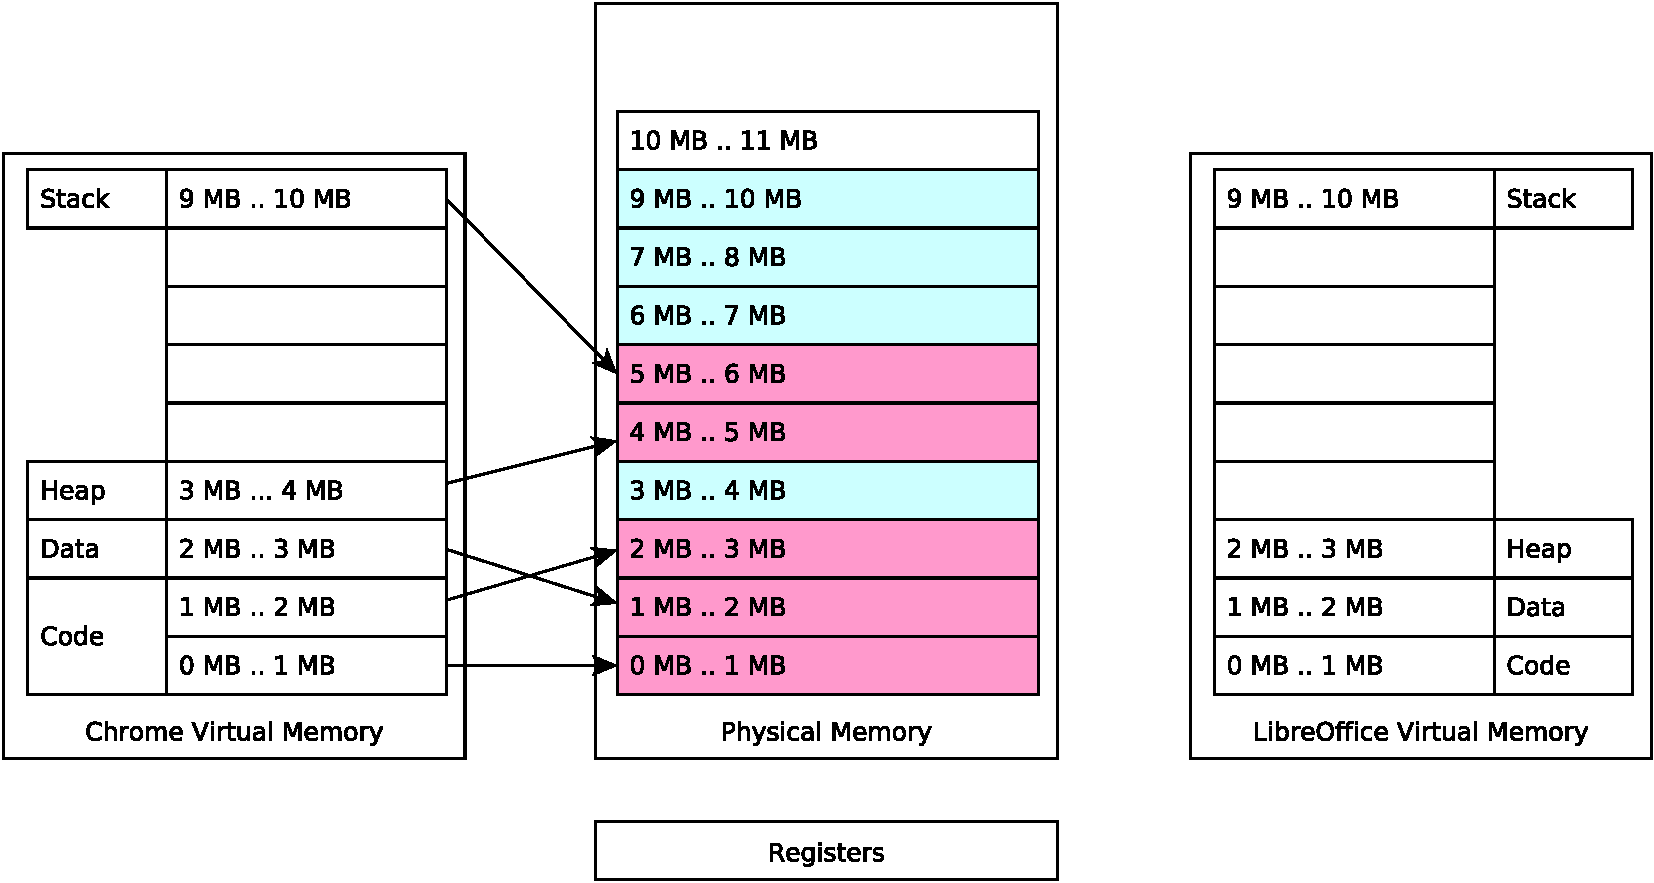
\includegraphics[width=0.9\linewidth]{ctx1}
}
    \only<2> {
  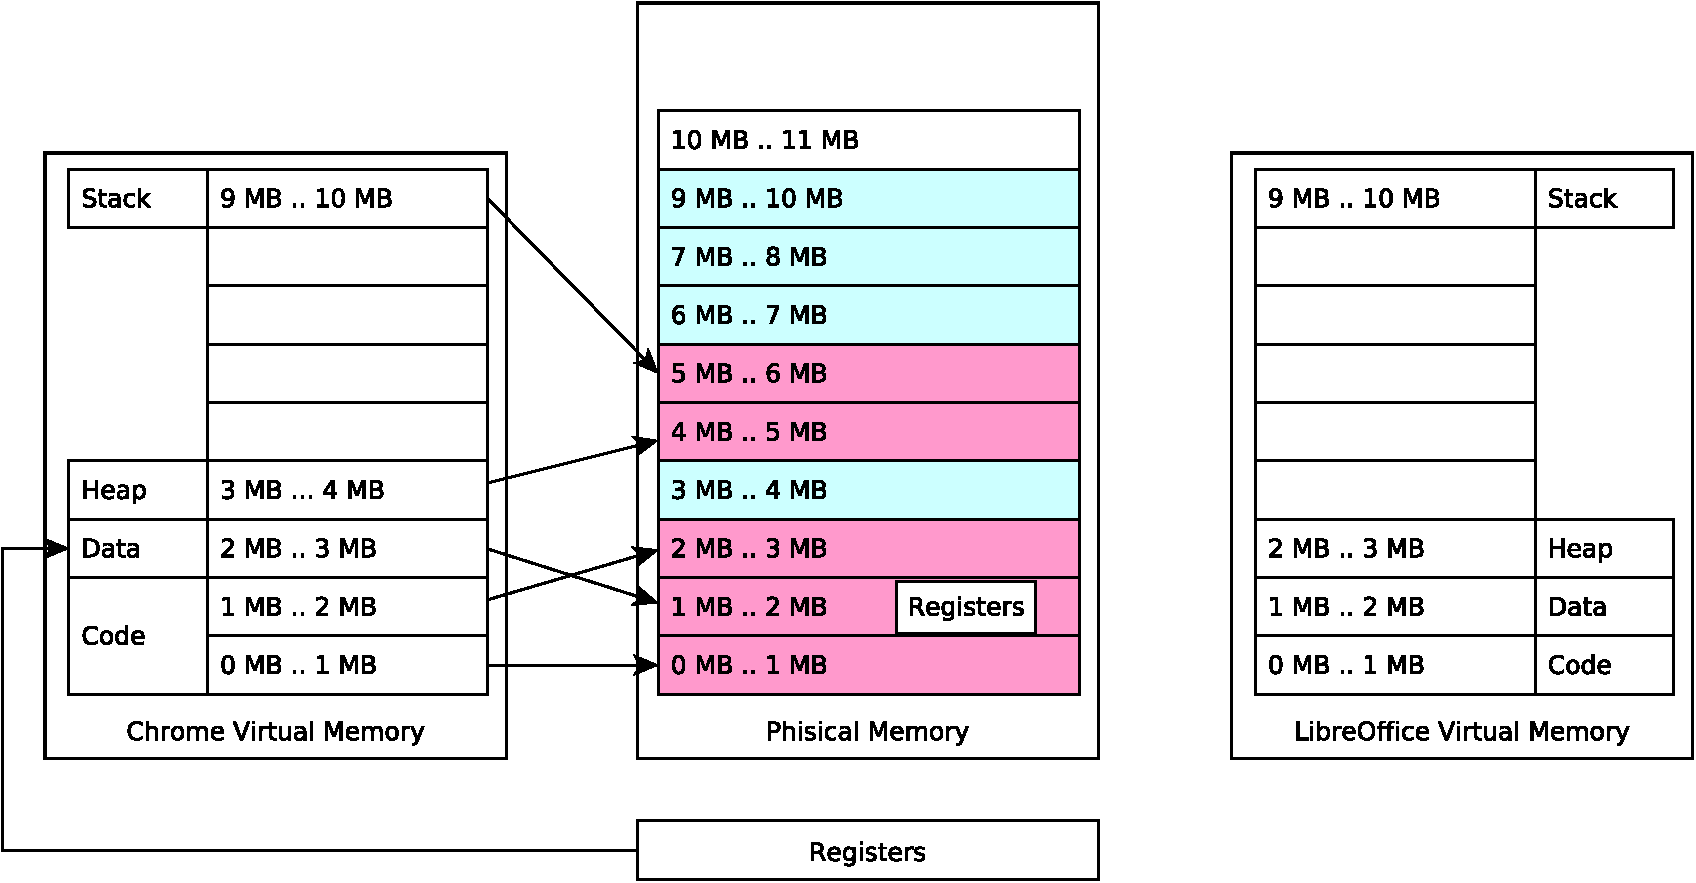
\includegraphics[width=0.9\linewidth]{ctx2}
}
    \only<3> {
  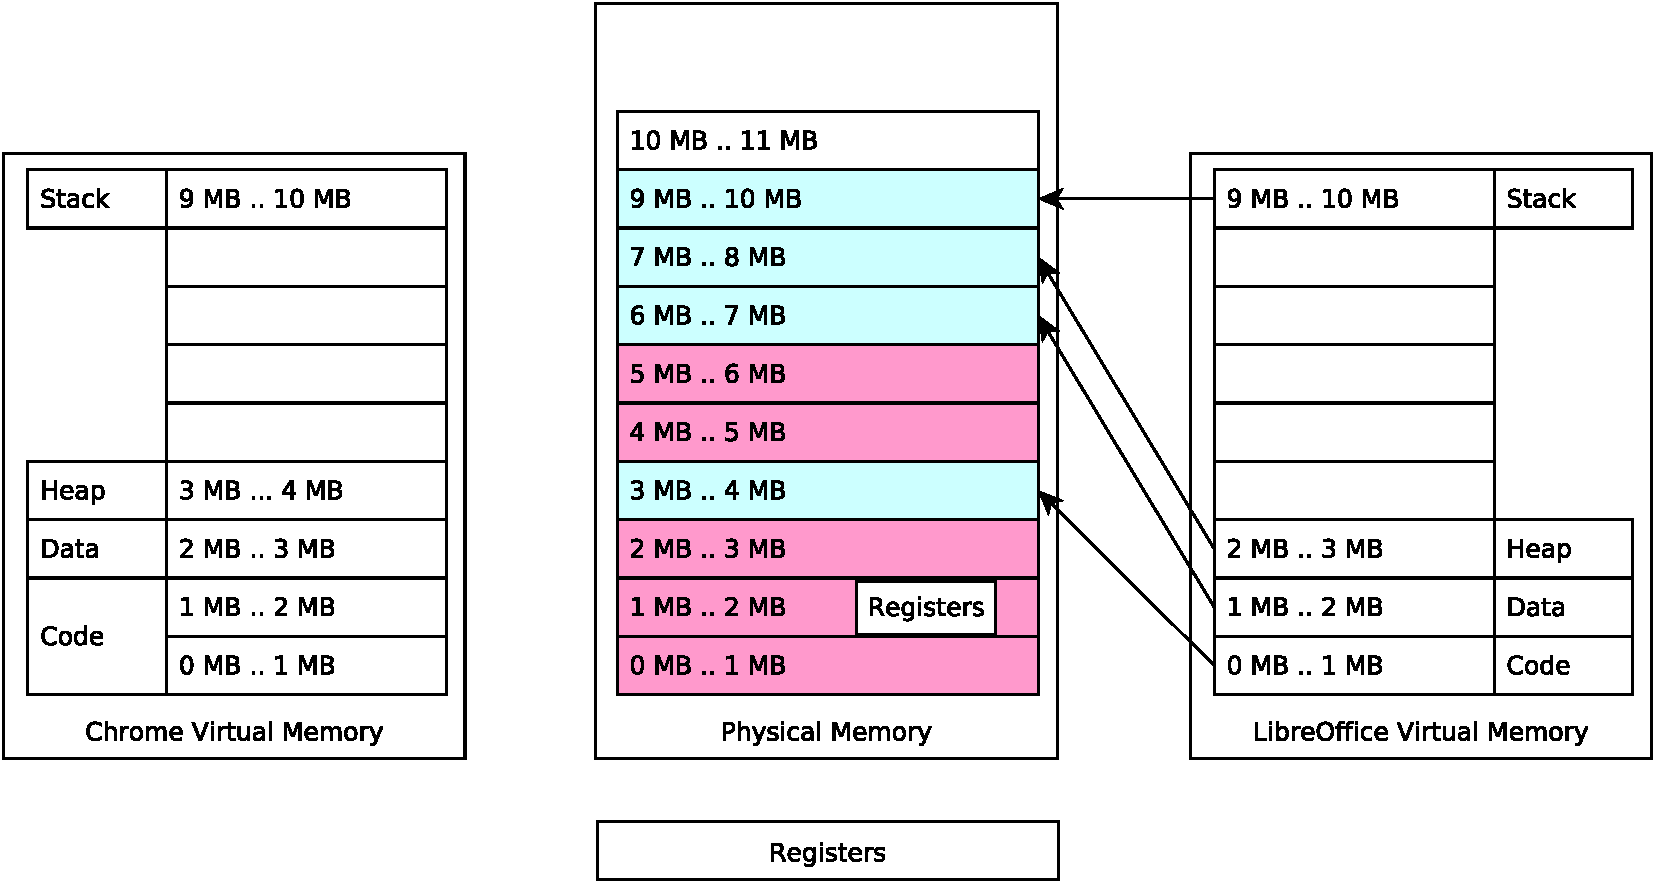
\includegraphics[width=0.9\linewidth]{ctx3}
}
    \only<4> {
  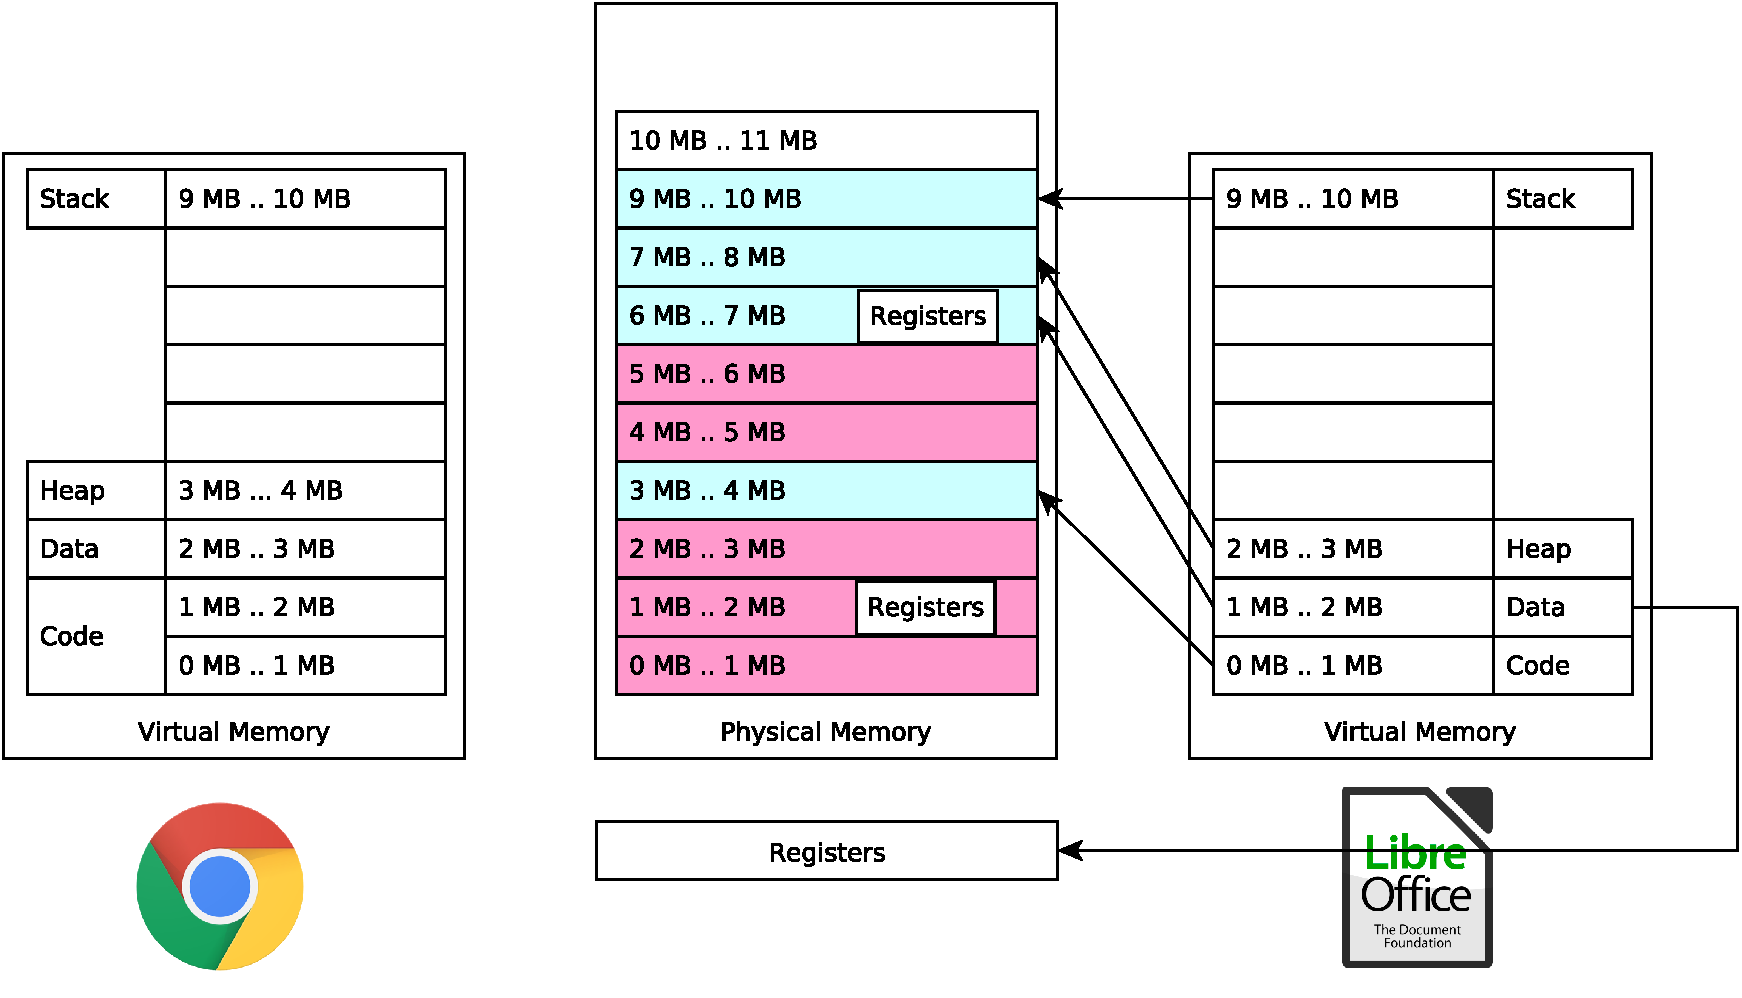
\includegraphics[width=0.9\linewidth]{ctx4}
}
  \end{center}
\end{frame}






\begin{frame}{HW architecture}
  \begin{itemize}
  \item Privilege level (i.e. Ring 3/Ring 0, PL1/PL0, CPU modes)
  \item OS takes control of privileged level
  \item Everything else uses non-privileged level
  \end{itemize}
  \begin{center}
  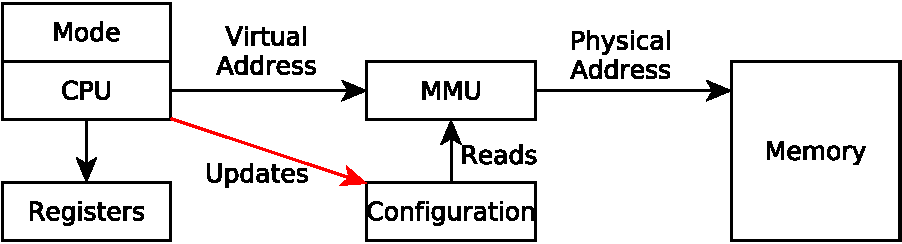
\includegraphics[width=0.5\linewidth]{mode0}
  \end{center}
  \begin{itemize}
  \item<2-> From PL1 to PL0 = exiting the OS
  \begin{itemize}
    \item instruction to change mode
  \end{itemize}
  \item<3-> From PL0 to PL1 = entering the OS? \alert{Question?}
  \begin{itemize}
    \item<4-> interrupts
  \end{itemize}
  \end{itemize}
\end{frame}



\begin{frame}{SW interrupt}
  \begin{enumerate}
  \item<1-> Application executes the Software Interrupt Instruction
  \item<2-> HW
  \begin{itemize}
    \item Mode switches to privileged
    \item Program counter jumps to the OS \alert{vector table}
  \end{itemize}
  \item<3-> OS
  \begin{itemize}
    \item Saves the registers (context) in the process memory
    \item Jumps to the \alert{exception handler}
    \item \dots \\
 (e.g. change MMU configuration and ``logical'' active process)
    \item Loads the registers (context) from the memory of the  \alert{active}
      process
  \end{itemize}
  \item<4-> Context switch driven by software interrupt $\Rightarrow$\\
    Cooperative/non-preemptive multitasking
\end{enumerate}
\end{frame}

\begin{frame}{HW Interrupt}
  \begin{center}
  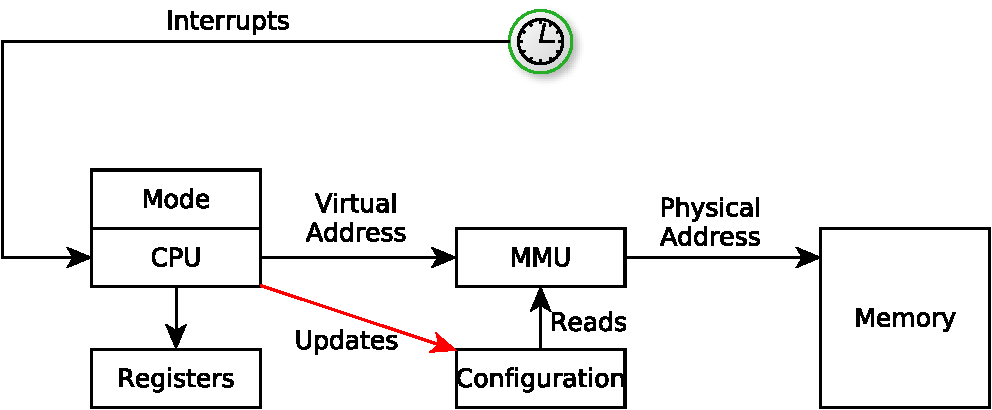
\includegraphics[width=0.5\linewidth]{timer}
  \end{center}
  \begin{enumerate}
  \item<1-> Peripheral (timer) delivers an Hardware Interrupt
  \item<2-> HW
  \begin{itemize}
    \item Mode switches to privileged
    \item Program counter jumps to the OS ``vector table''
  \end{itemize}
  \item<3-> OS
  \begin{itemize}
    \item Saves the registers (context) in the process memory
    \item Jumps to the ``exception handler''
    \item \dots \\
 (e.g. change MMU configuration and ``logical'' active process)
    \item Loads the registers (context) from the memory of the  \alert{active}
      process
  \end{itemize}
  \item<4-> Preemptive multitasking
\end{enumerate}
\end{frame}


\begin{frame}{OS Memory}
  \begin{enumerate}
  \item<1-> How does the OS access the memory?
  \item<2-> Virtual memory
  \item<7-> MMU enforces access right
\end{enumerate}
\begin{center}
\only<3>{
  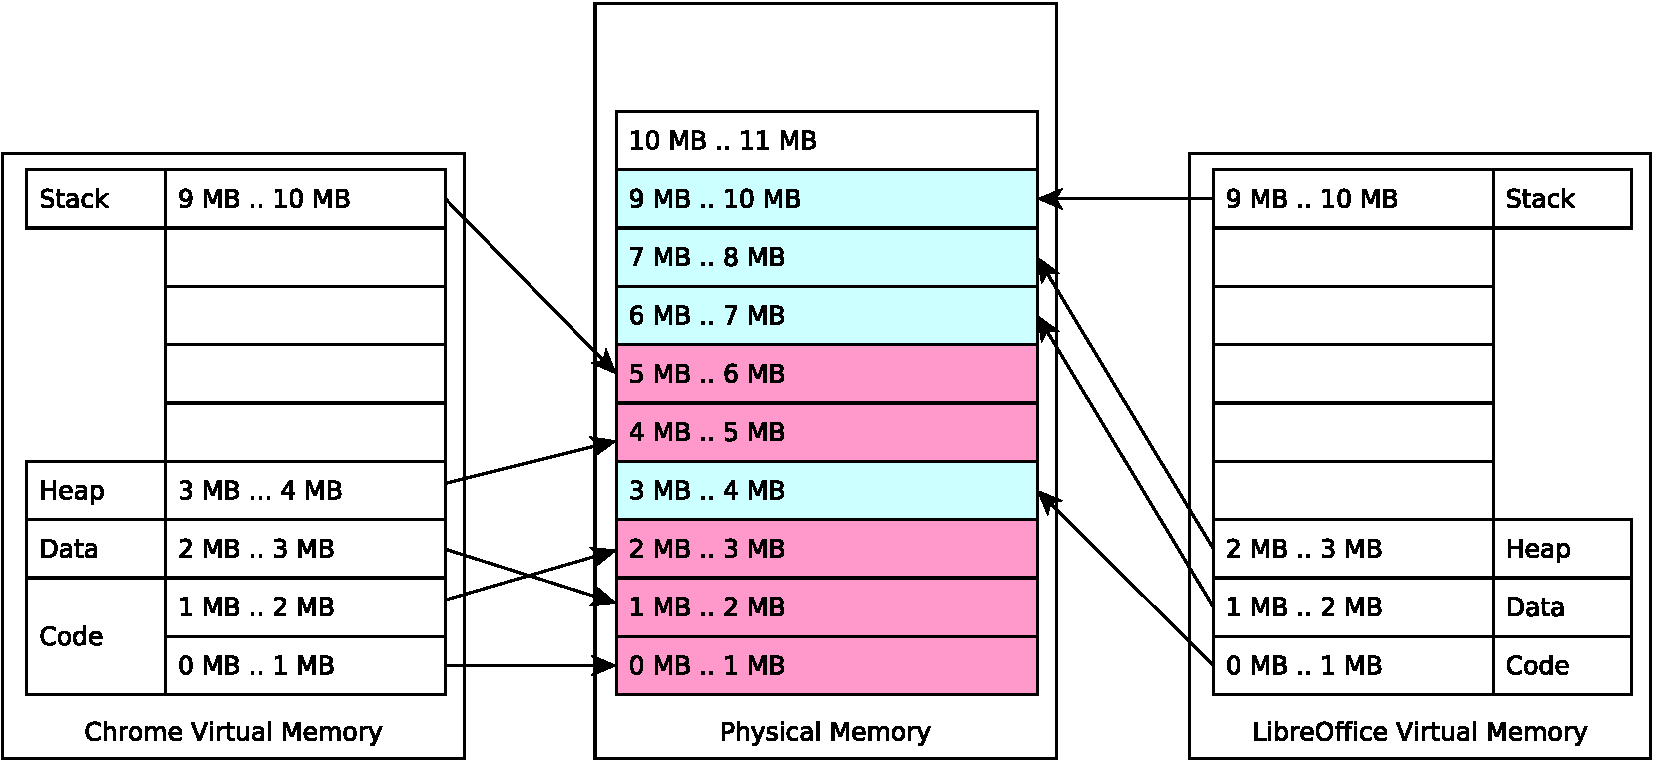
\includegraphics[width=0.8\linewidth]{ctx0}
}
\only<4>{
  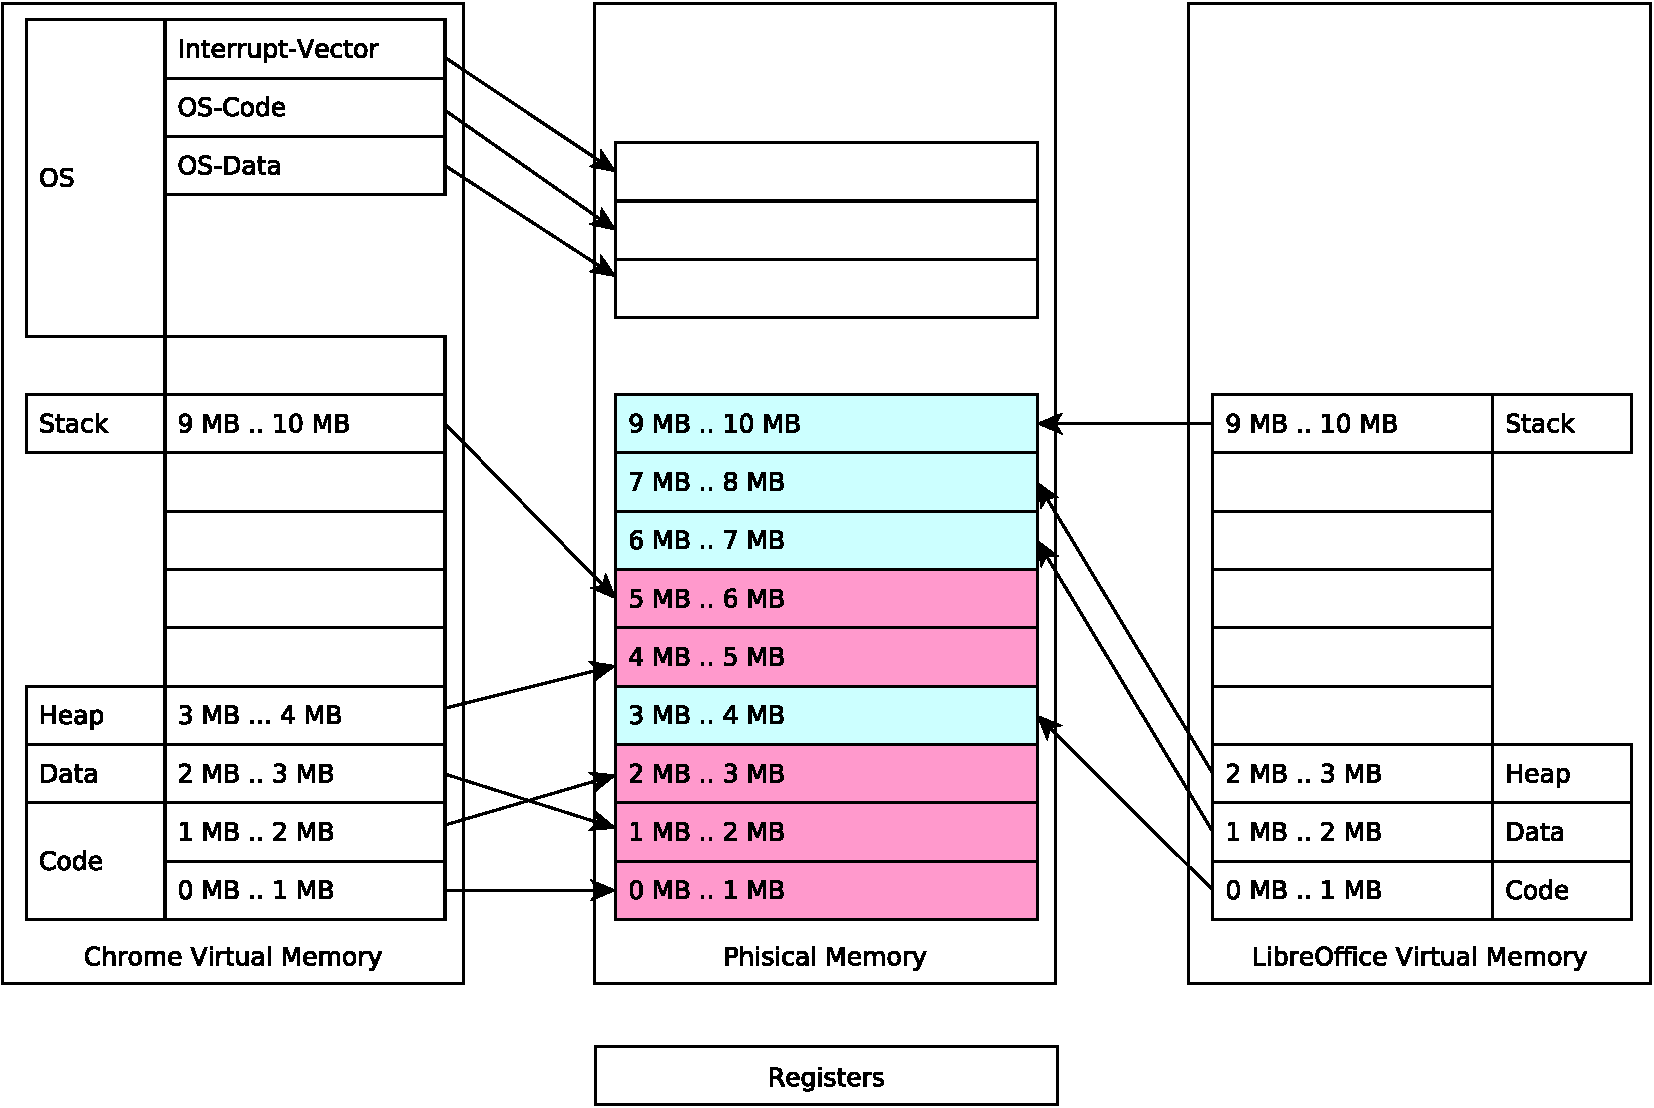
\includegraphics[width=0.8\linewidth]{os-mem-0}
}
\only<5>{
  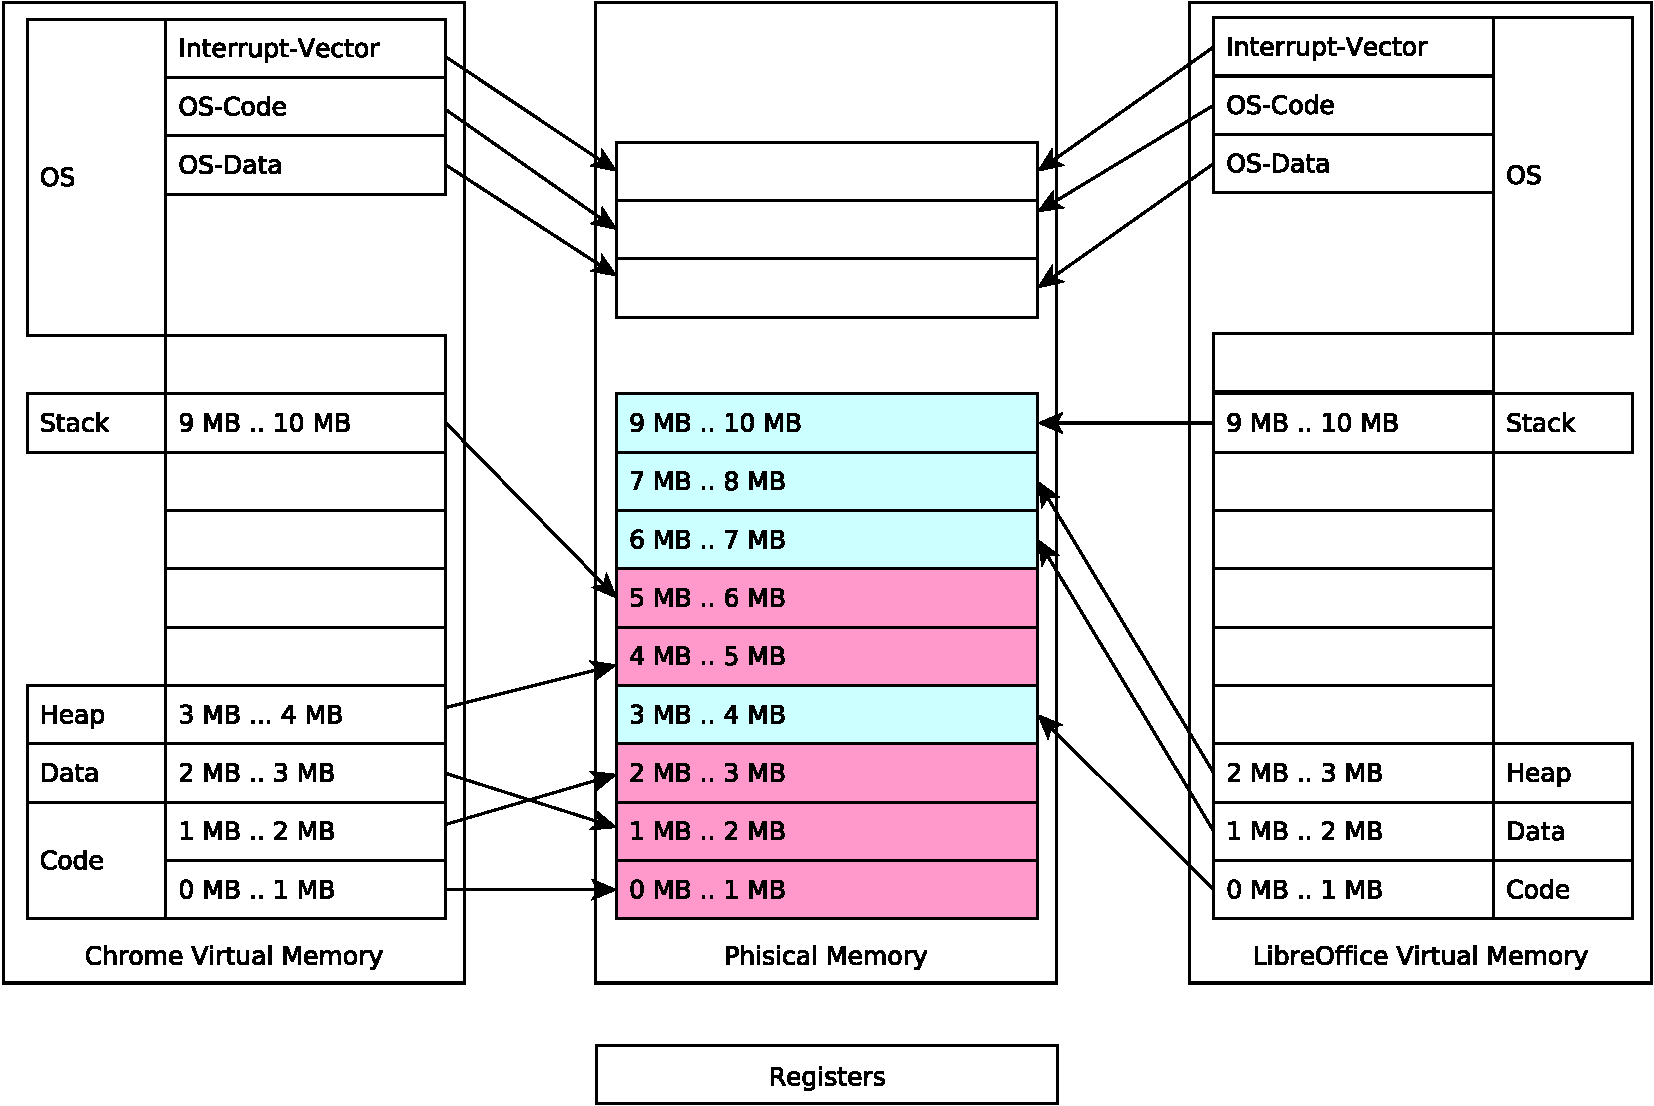
\includegraphics[width=0.8\linewidth]{os-mem-1}
}
\only<6>{
  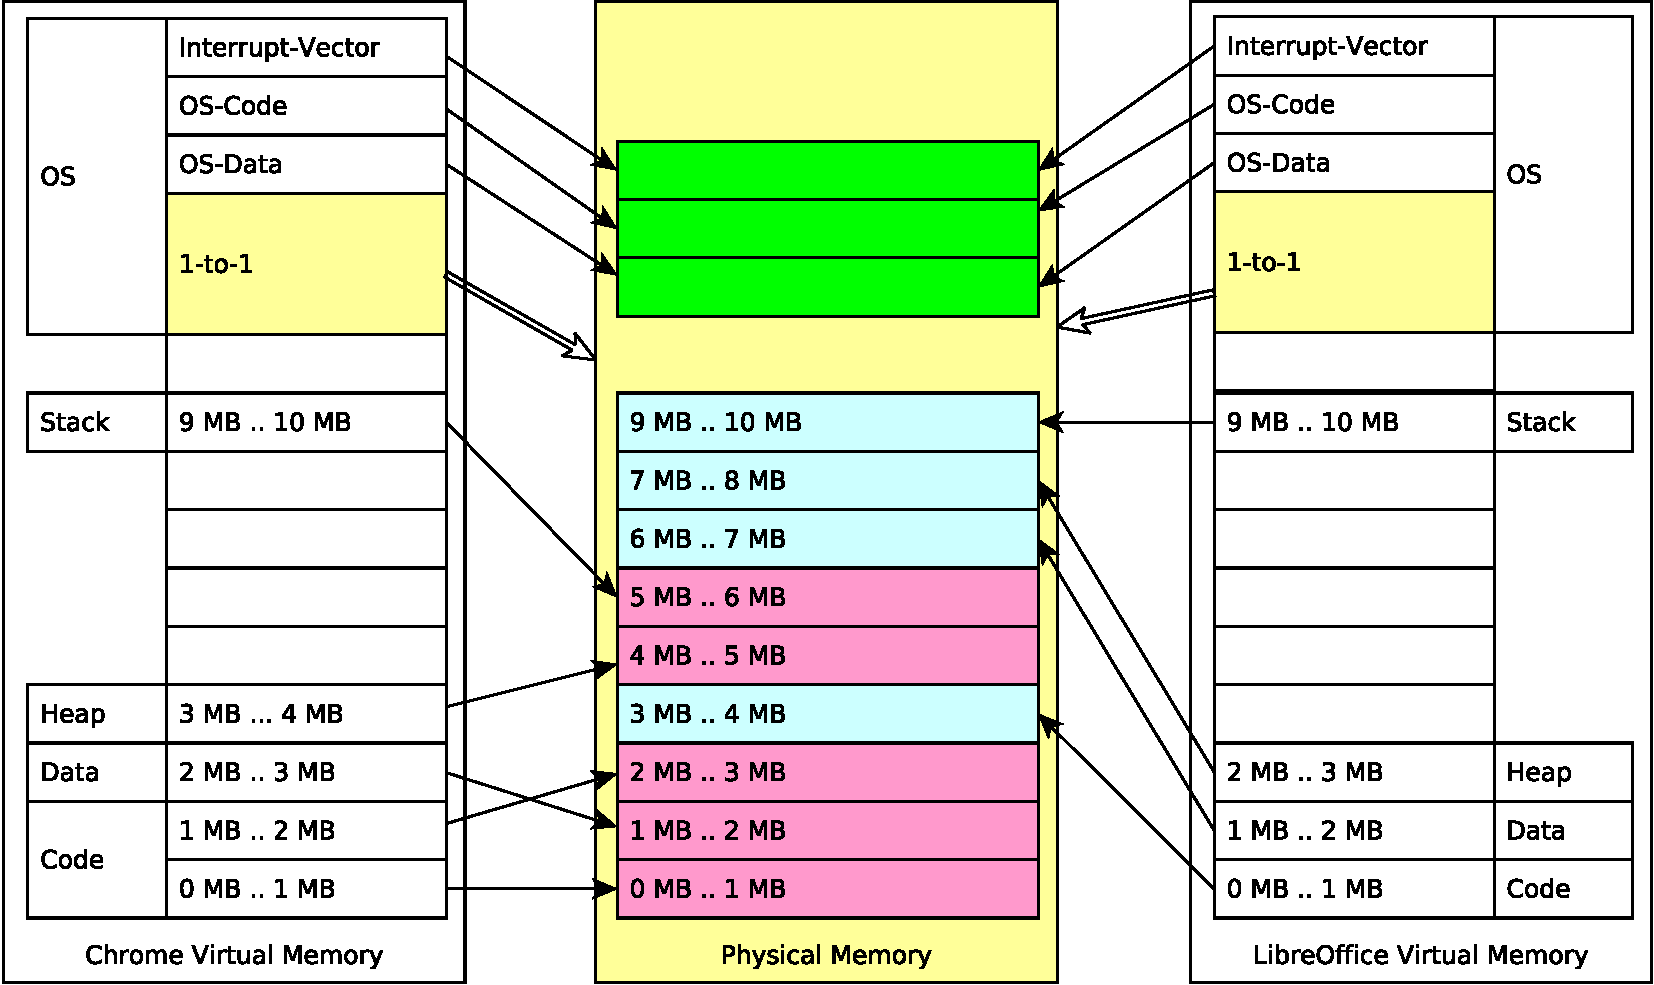
\includegraphics[width=0.8\linewidth]{os-mem-2}
}
\only<7>{
  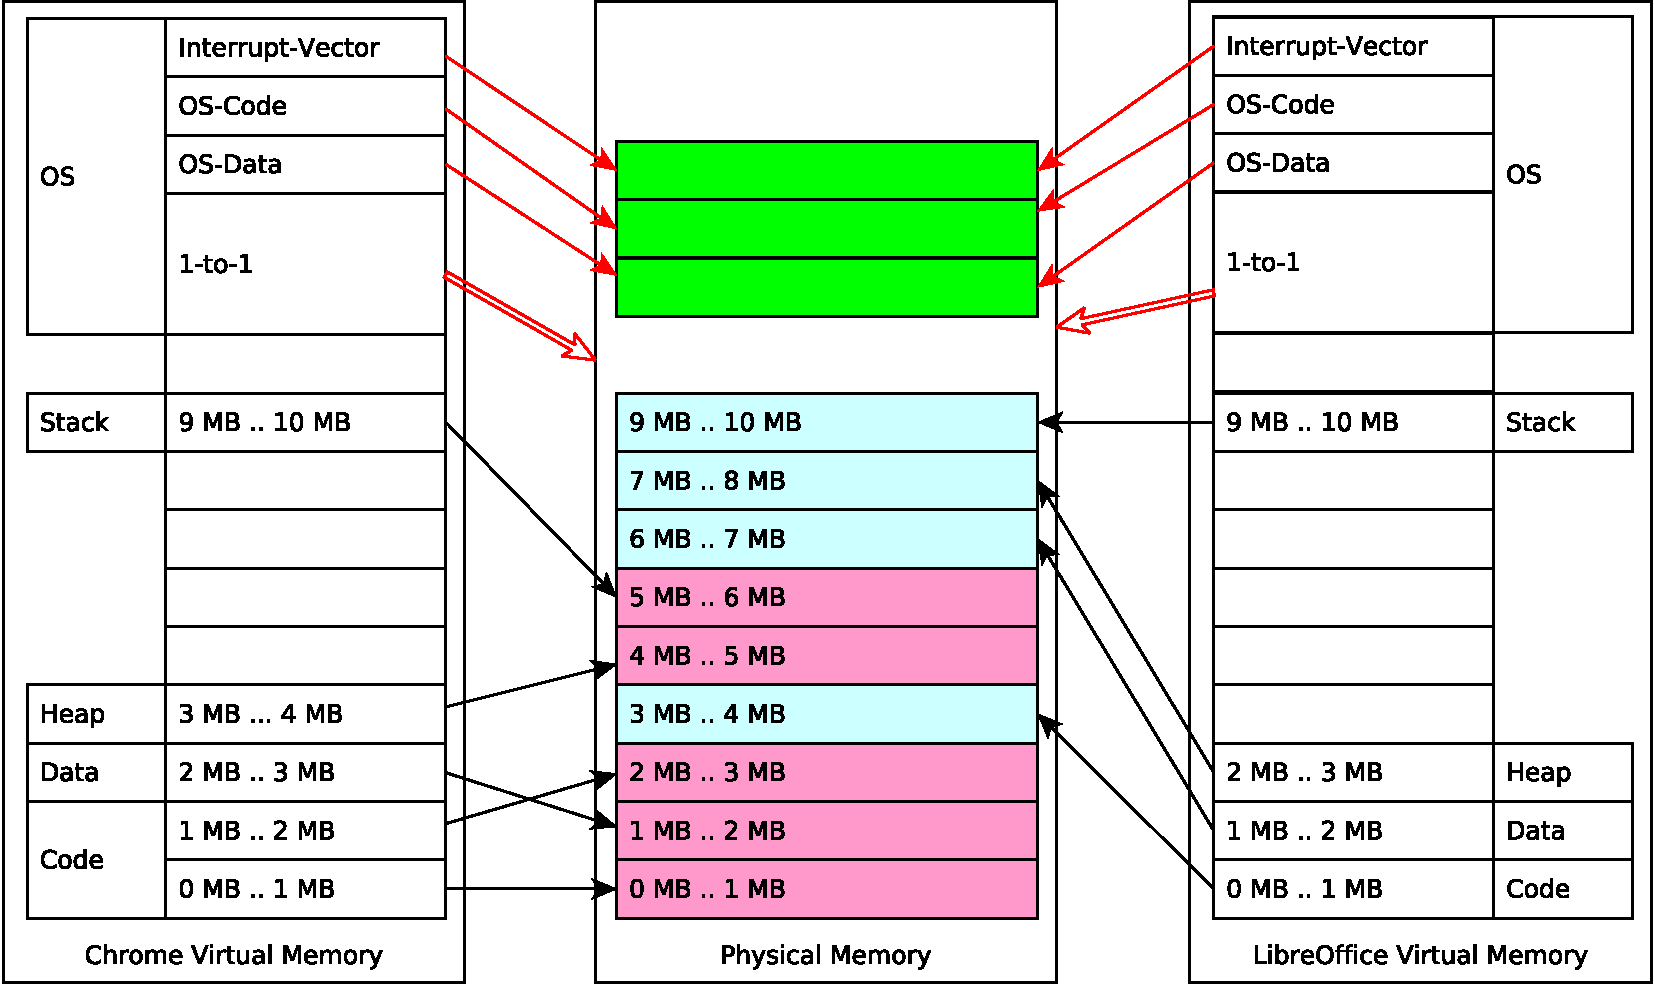
\includegraphics[width=0.8\linewidth]{os-mem-3}
}
\end{center}
\end{frame}

\begin{frame}[t]{Peripherals}
  \begin{enumerate}
  \item<1-> Interrupts
  \item<2-> Memory mapped devices
  \item<4-> Direct Memory Access
\end{enumerate}
\begin{center}
\only<1>{
  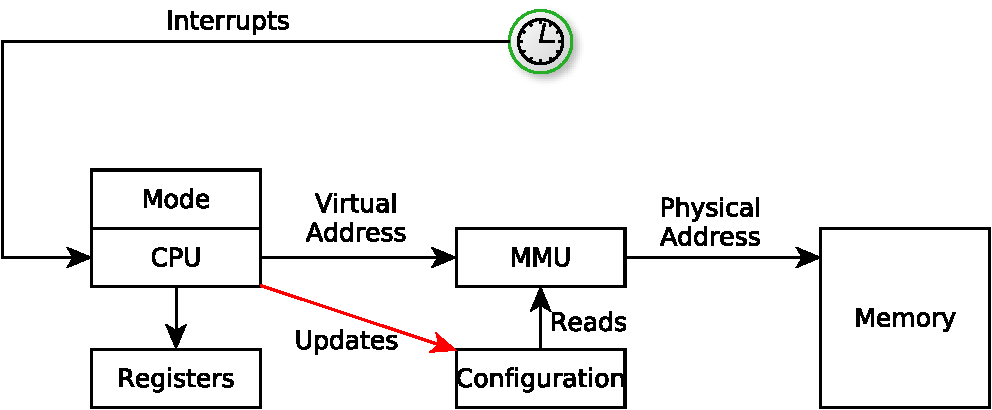
\includegraphics[width=0.8\linewidth]{timer}
}
\only<2>{
  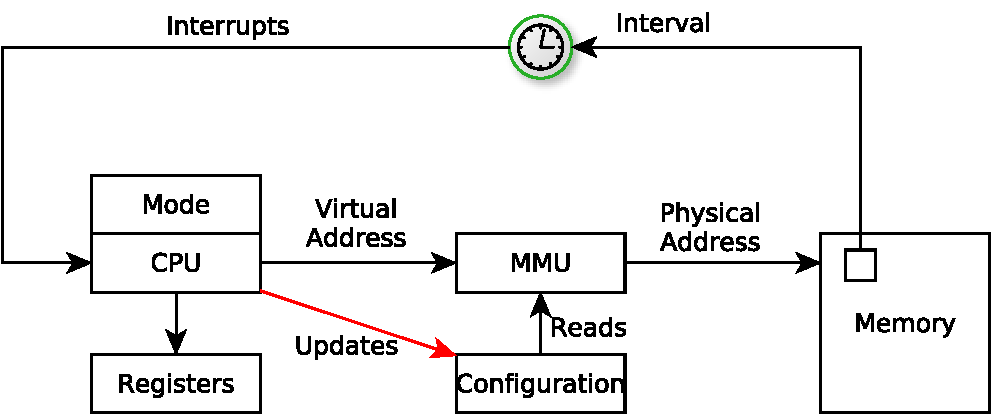
\includegraphics[width=0.8\linewidth]{timer1}
}
\only<3>{
  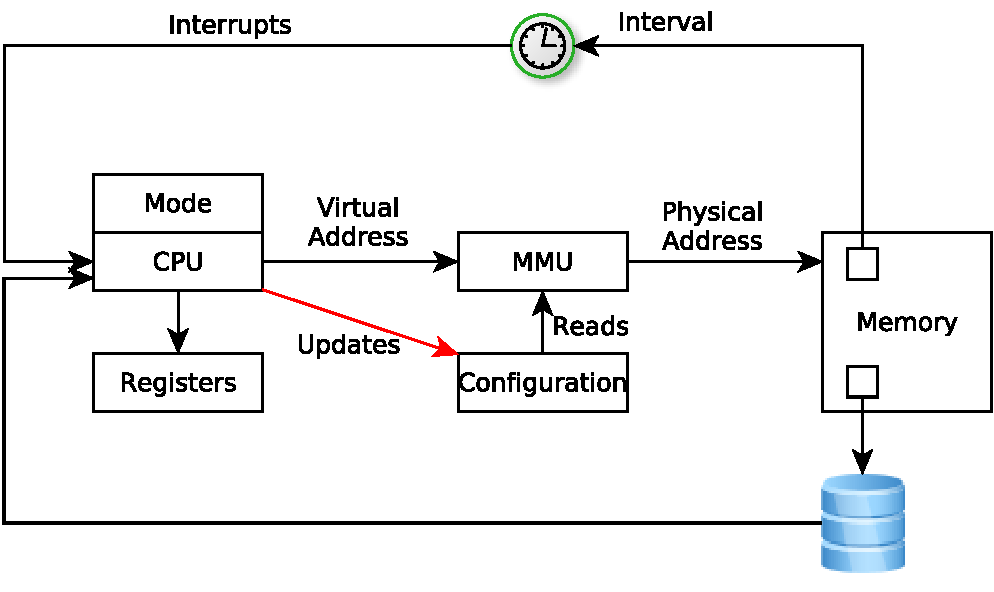
\includegraphics[width=0.8\linewidth]{dev1}
}
\only<4>{
  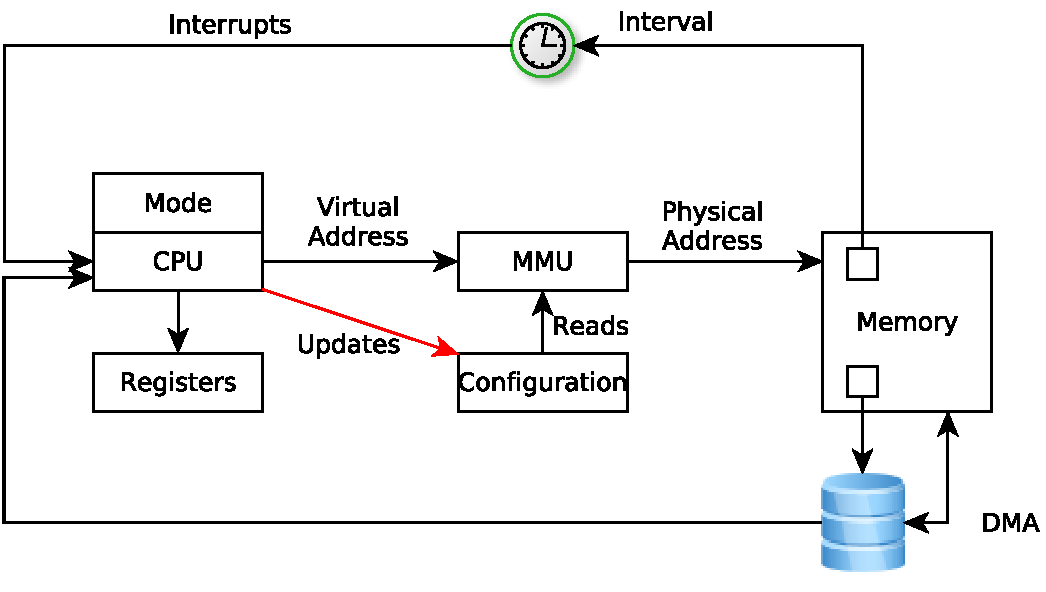
\includegraphics[width=0.85\linewidth]{dev2}
}
\only<5>{
  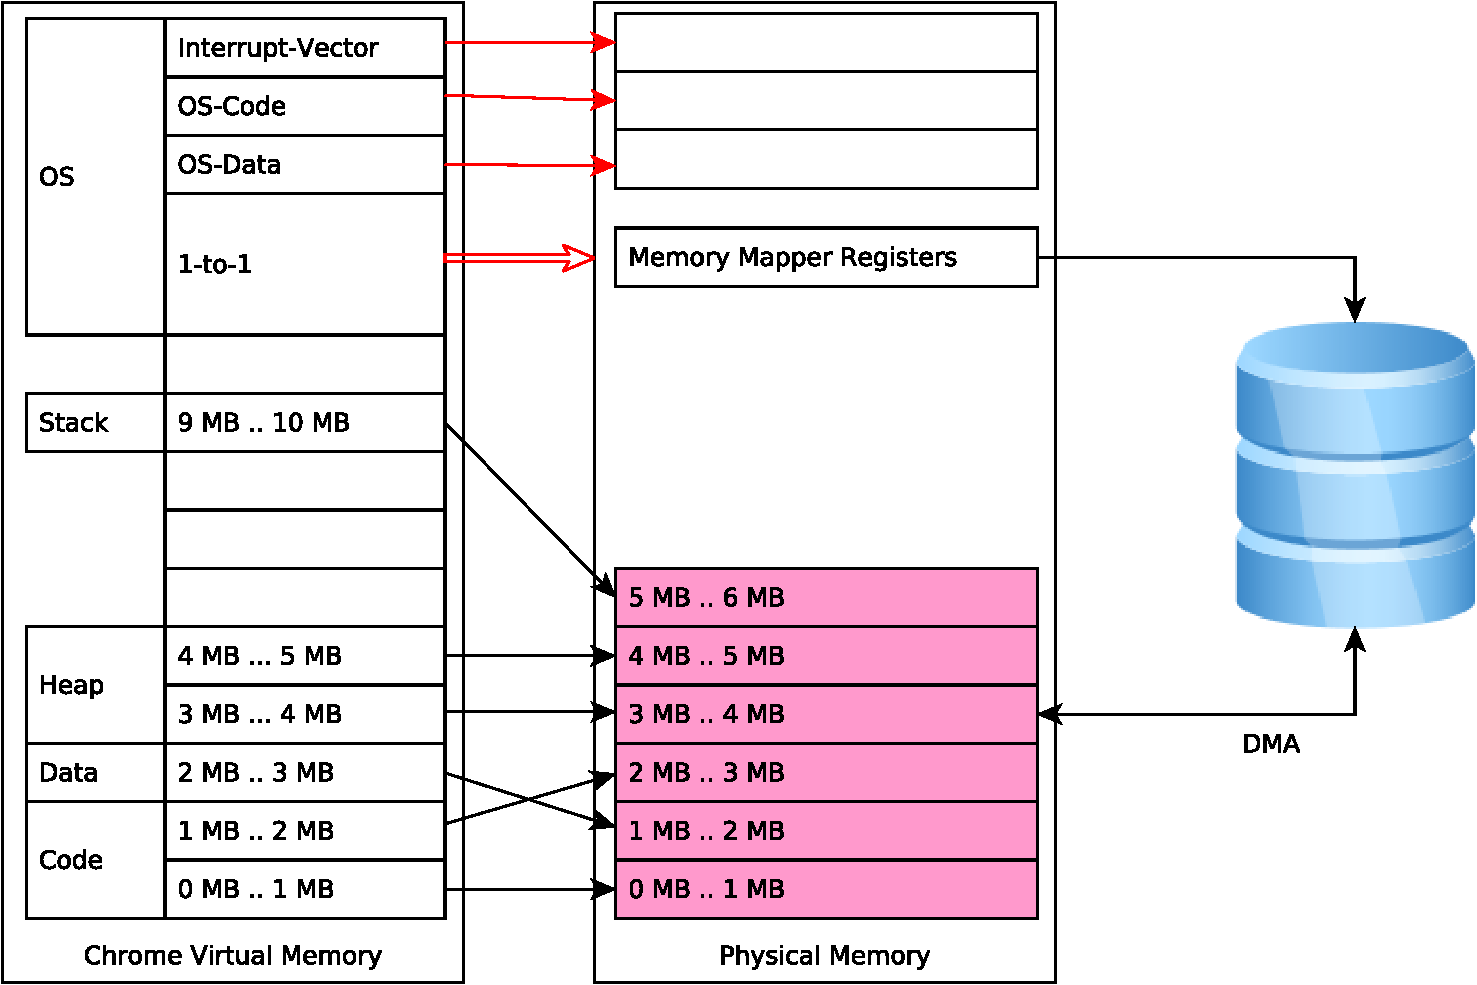
\includegraphics[width=0.7\linewidth]{dma}
}
\end{center}
\end{frame}

\begin{frame}{OS blocks}
\begin{center}
\only<1>{
  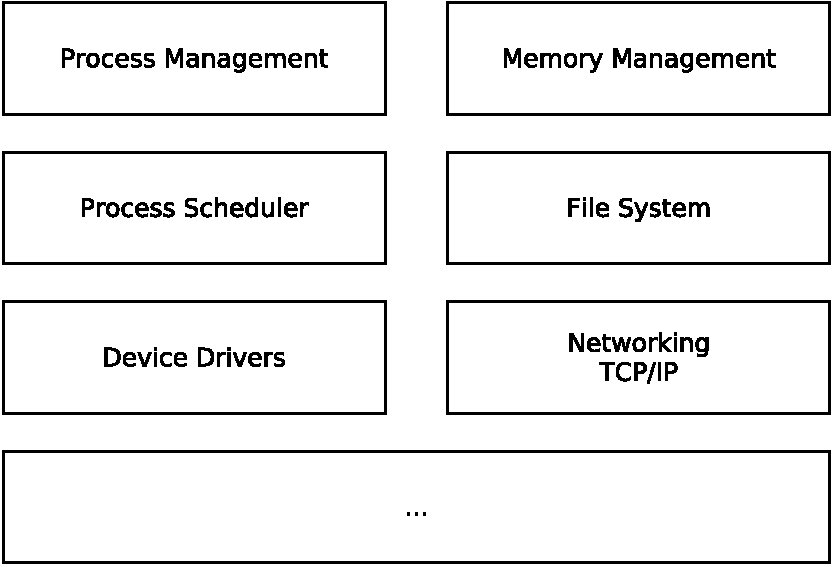
\includegraphics[width=0.8\linewidth]{os-blocks}
}
\only<2>{
  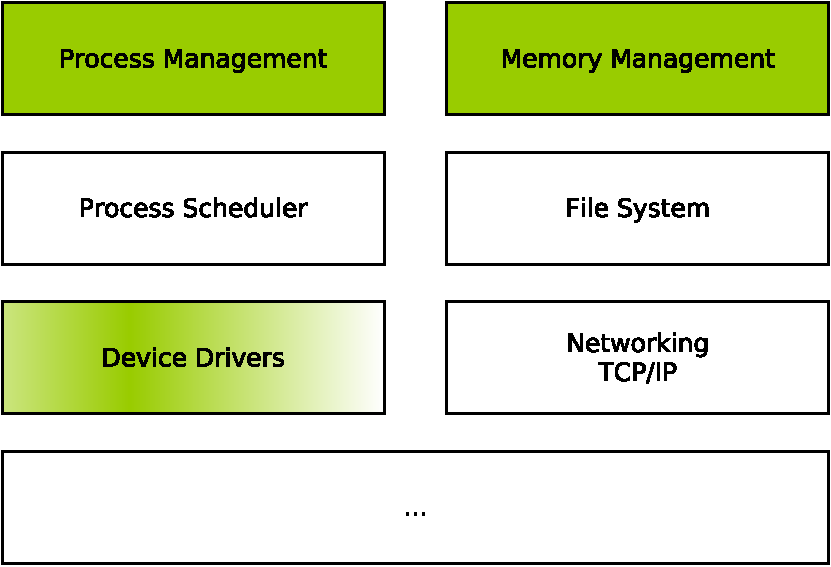
\includegraphics[width=0.8\linewidth]{os-block-2}
}
\end{center}
\end{frame}






\begin{frame}{System calls}
    \begin{itemize}
      \item Request OS services
    \begin{itemize}
      \item \alert<2>{File management}
      \item Device Management
      \item Memory allocation
      \item Process Control
      \item Communication
      \item Print to the terminal
   \end{itemize}
   \item Calling convention
    \begin{itemize}
    \item Usually invoked by Software Interrupts
    \item HW-OS dependent
   \end{itemize}
   \end{itemize}
\end{frame}

\begin{frame}{OS API}
    \begin{itemize}
    \item Syscall low level (and non-portable)
    \item Library or API that sits between normal programs and the
      operating system 
    \item Unix-like: libc, glibc
    \item Windows NT, that API is part of the Native API, in the
      ntdll.dll library
    \item in POSIX: open, read, write, close, wait, exec, fork, exit, mmap
    \end{itemize}
\end{frame}


\begin{frame}{Shared memory}
\begin{center}
\only<1>{
  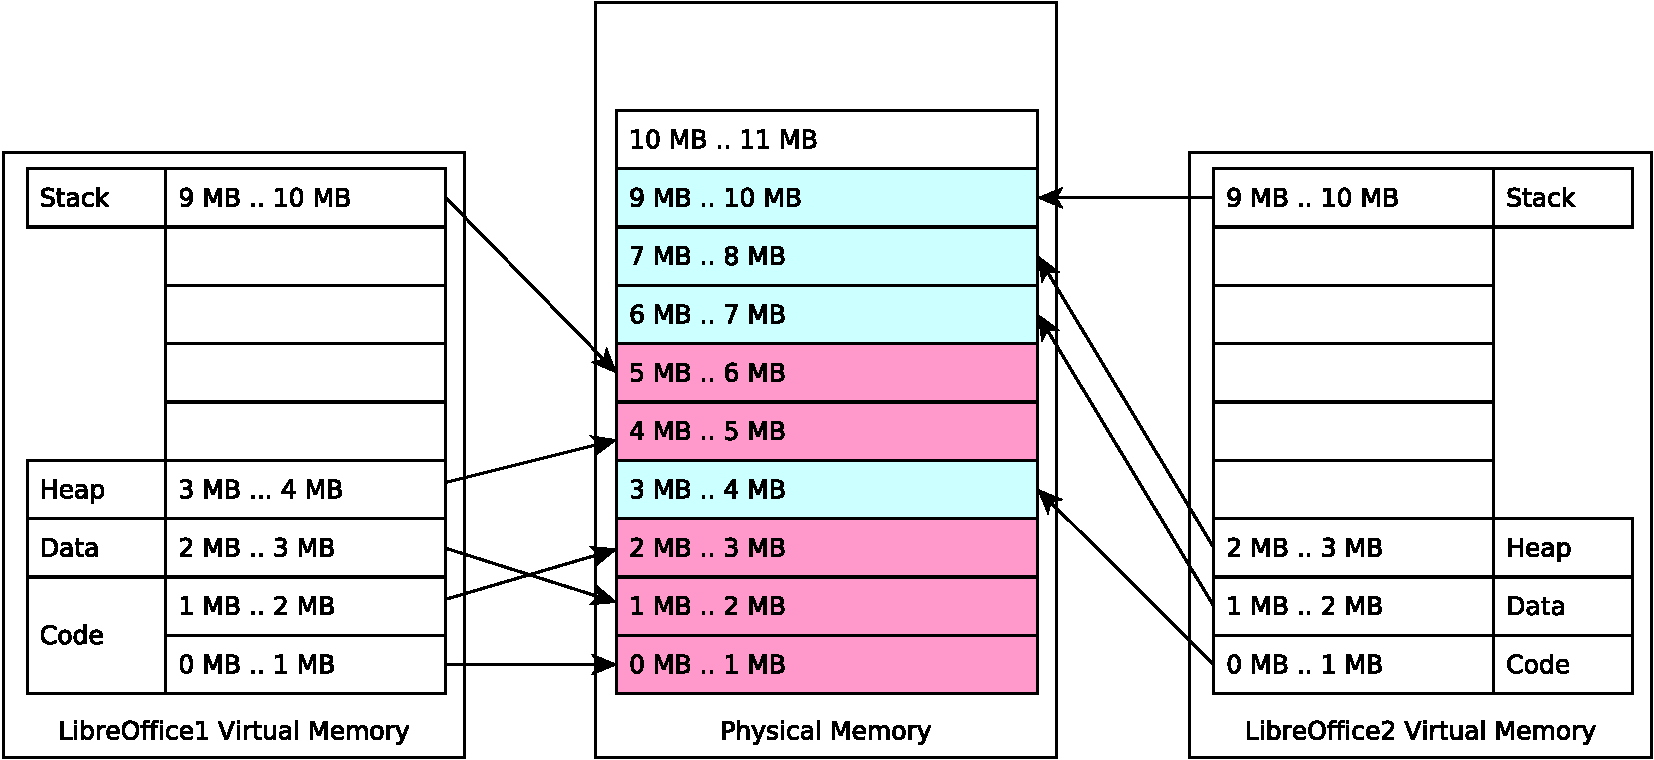
\includegraphics[width=0.9\linewidth]{2libre-0}
}
\only<2>{
  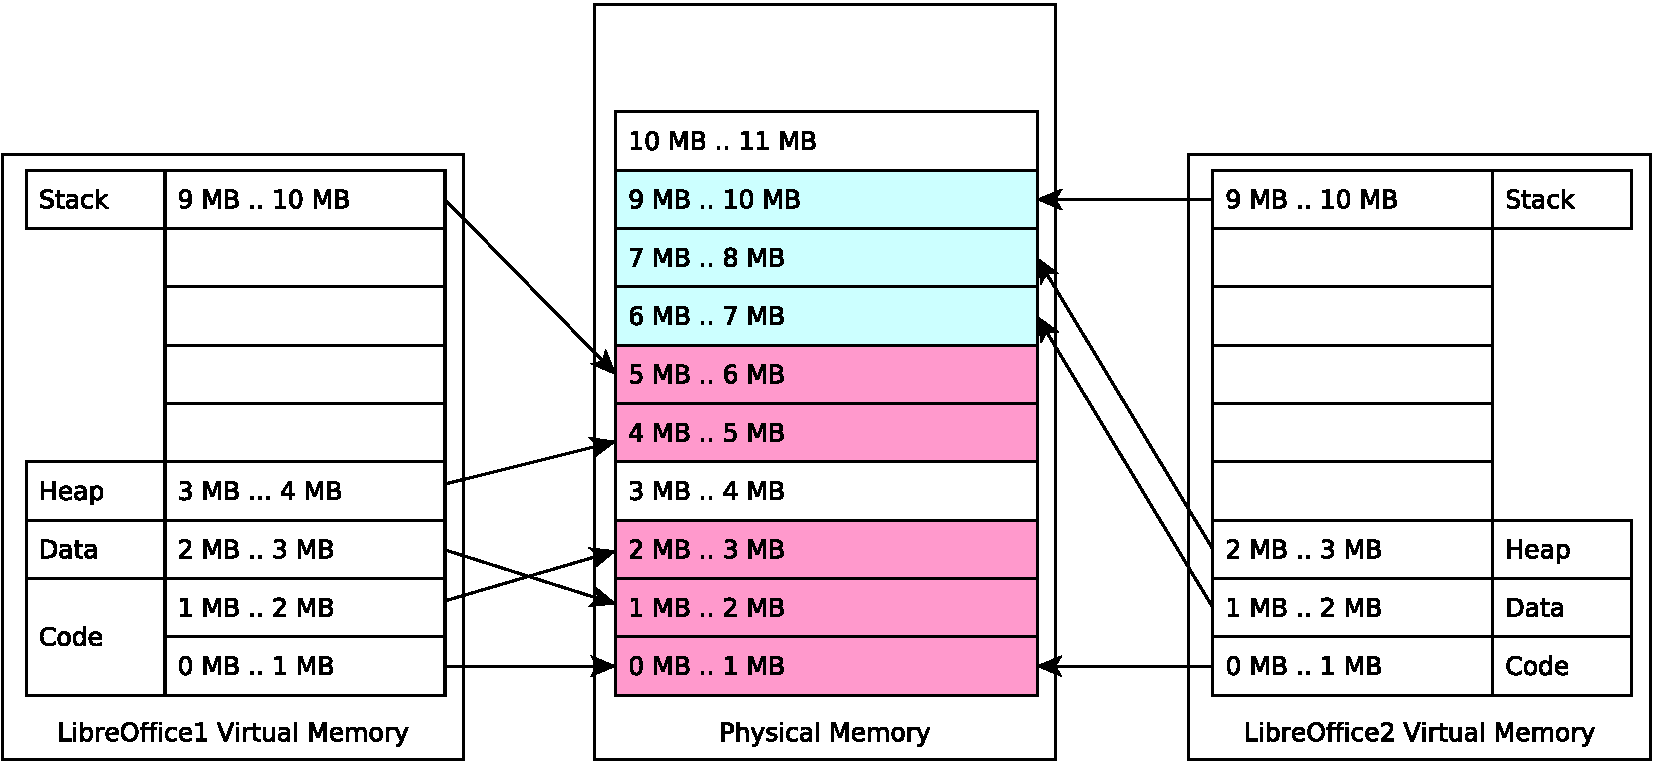
\includegraphics[width=0.9\linewidth]{2libre-1}
}
\end{center}
\end{frame}

\begin{frame}{Executing a new process}
\end{frame}

\begin{frame}{Questions?}
    Questions?
\end{frame}

\end{document}
